%% tikz-3dplot_documentation.tex
%% Copyright 2010-2012 Jeffrey D. Hein
%
% This work may be distributed and/or modified under the
% conditions of the LaTeX Project Public License, either version 1.3
% of this license or (at your option) any later version.
% The latest version of this license is in
%   http://www.latex-project.org/lppl.txt
% and version 1.3 or later is part of all distributions of LaTeX
% version 2005/12/01 or later.
%
% This work has the LPPL maintenance status `maintained'.
% 
% The Current Maintainer of this work is Jeffrey D. Hein.
%
% This work consists of the files tikz-3dplot.sty and tikz-3dplot_documentation.tex

%Description
%-----------

%tikz-3dplot_documentation.tex - documentation for tikz-3dplot.sty: package for plotting three dimensional axes and coordinates in TikZ.  The user can specify orientation of the display, and also define rotated coordinate systems within the 3d display coordinate system.  

%Created 2009-11-07 by Jeff Hein.  Last updated: 2010-07-30
%----------------------------------------------------------

%Requirements
%------------
%This requires the tikz package.

%Update Notes
%------------

%As of Jan 17, 2010, this package has been renamed from ``3dplot'' to ``tikz-3dplot''.


\documentclass[10pt,letterpaper,oneside]{memoir}

\usepackage{tikz}			%for TikZ graphics
\usepackage{tikz-3dplot} %for tikz-3dplot functionality
\usepackage{amsmath}		%for align equation environment
\usepackage{url}

\pgfrealjobname{tikz-3dplot_documentation}

\usepackage[pdftex]{hyperref}
\hypersetup{pdftitle={The tikz-3dplot Package}}
\hypersetup{pdfauthor={Jeff Hein}}
\hypersetup{pdfsubject={LaTeX}}
\hypersetup{pdfcreator={Jeff Hein}}
\hypersetup{colorlinks=true}
\hypersetup{citecolor=darkgreen}



\newcommand{\tdplotmainfig}{%
%Angle Definitions
%-----------------
%
%set the plot display orientation
%synatax: \tdplotsetdisplay{\theta_d}{\phi_d}
\tdplotsetmaincoords{60}{110}
%
%define polar coordinates for some vector
%TODO: look into using 3d spherical coordinate system
\pgfmathsetmacro{\rvec}{.8}
\pgfmathsetmacro{\thetavec}{30}
\pgfmathsetmacro{\phivec}{60}
%
%start tikz picture, and use the tdplot_main_coords style to implement the display coordinate transformation provided by 3dplot
\begin{tikzpicture}[scale=3,tdplot_main_coords]

	%set up some coordinates 
	%-----------------------
	\coordinate (O) at (0,0,0);

	%determine a coordinate (P) using (r,\theta,\phi) coordinates.  This command also determines (Pxy), (Pxz), and (Pyz): the xy-, xz-, and yz-projections of the point (P).
	%synatax: \tdplotsetcoord{Coordinate name without parentheses}{r}{\theta}{\phi}
	\tdplotsetcoord{P}{\rvec}{\thetavec}{\phivec}

	%draw figure contents
	%--------------------

	%draw the main coordinate system axes
	\draw[thick,->] (0,0,0) -- (1,0,0) node[anchor=north east]{$x$};
	\draw[thick,->] (0,0,0) -- (0,1,0) node[anchor=north west]{$y$};
	\draw[thick,->] (0,0,0) -- (0,0,1) node[anchor=south]{$z$};

	%draw a vector from origin to point (P) 
	\draw[-stealth,color=red] (O) -- (P);

	%draw projection on xy plane, and a connecting line
	\draw[dashed, color=red] (O) -- (Pxy);
	\draw[dashed, color=red] (P) -- (Pxy);

	%draw the angle \phi, and label it
	%syntax: \tdplotdrawarc[coordinate frame, draw options]{center point}{r}{angle}{label options}{label}
	\tdplotdrawarc{(O)}{0.2}{0}{\phivec}{anchor=north}{$\phi$}


	%set the rotated coordinate system so the x'-y' plane lies within the "theta plane" of the main coordinate system
	%syntax: \tdplotsetthetaplanecoords{\phi}
	\tdplotsetthetaplanecoords{\phivec}

	%draw theta arc and label, using rotated coordinate system
	\tdplotdrawarc[tdplot_rotated_coords]{(0,0,0)}{0.5}{0}{\thetavec}{anchor=south west}{$\theta$}

	%draw some dashed arcs, demonstrating direct arc drawing
	\draw[dashed,tdplot_rotated_coords] (\rvec,0,0) arc (0:90:\rvec);
	\draw[dashed] (\rvec,0,0) arc (0:90:\rvec);

	%set the rotated coordinate definition within display using a translation coordinate and Euler angles in the "z(\alpha)y(\beta)z(\gamma)" euler rotation convention
	%syntax: \tdplotsetrotatedcoords{\alpha}{\beta}{\gamma}
	\tdplotsetrotatedcoords{\phivec}{\thetavec}{0}

	%translate the rotated coordinate system
	%syntax: \tdplotsetrotatedcoordsorigin{point}
	\tdplotsetrotatedcoordsorigin{(P)}

	%use the tdplot_rotated_coords style to work in the rotated, translated coordinate frame
	\draw[thick,tdplot_rotated_coords,->] (0,0,0) -- (.5,0,0) node[anchor=north west]{$x'$};
	\draw[thick,tdplot_rotated_coords,->] (0,0,0) -- (0,.5,0) node[anchor=west]{$y'$};
	\draw[thick,tdplot_rotated_coords,->] (0,0,0) -- (0,0,.5) node[anchor=south]{$z'$};

	%WARNING:  coordinates defined by the \coordinate command (eg. (O), (P), etc.) cannot be used in rotated coordinate frames.  Use only literal coordinates.  

	%draw some vector, and its projection, in the rotated coordinate frame
	\draw[-stealth,color=blue,tdplot_rotated_coords] (0,0,0) -- (.2,.2,.2);
	\draw[dashed,color=blue,tdplot_rotated_coords] (0,0,0) -- (.2,.2,0);
	\draw[dashed,color=blue,tdplot_rotated_coords] (.2,.2,0) -- (.2,.2,.2);

	%show its phi arc and label
	\tdplotdrawarc[tdplot_rotated_coords,color=blue]{(0,0,0)}{0.2}{0}{45}{anchor=north west,color=black}{$\phi'$}

	%change the rotated coordinate frame so that it lies in its theta plane.  Note that this overwrites the original rotated coordinate frame
	%syntax: \tdplotsetrotatedthetaplanecoords{\phi'}
	\tdplotsetrotatedthetaplanecoords{45}

	%draw theta arc and label
	\tdplotdrawarc[tdplot_rotated_coords,color=blue]{(0,0,0)}{0.2}{0}{55}{anchor=south west,color=black}{$\theta'$}

\end{tikzpicture}
}

\newcommand{\threedcoord}[2]{%
\tdplotsetmaincoords{#1}{#2}
\begin{tikzpicture}[tdplot_main_coords]
	\draw[thick,->] (0,0,0) -- (1,0,0) node[anchor=north east]{$x$};
	\draw[thick,->] (0,0,0) -- (0,1,0) node[anchor=north west]{$y$};
	\draw[thick,->] (0,0,0) -- (0,0,1) node[anchor=south]{$z$};
\end{tikzpicture}
}

\newcommand{\threedrotcoordsystem}{%
\tdplotsetmaincoords{50}{140}
\begin{tikzpicture}[scale=5,tdplot_main_coords]
	\draw[thick,->] (0,0,0) -- (1,0,0) node[anchor=north east]{$x$};
	\draw[thick,->] (0,0,0) -- (0,1,0) node[anchor=north west]{$y$};
	\draw[thick,->] (0,0,0) -- (0,0,1) node[anchor=south]{$z$};

	\tdplotsetrotatedcoords{34}{26}{12}

	\draw[thick,color=blue,tdplot_rotated_coords,->] (0,0,0) -- (.5,0,0) node[anchor=north east]{$x'$};
	\draw[thick,color=blue,tdplot_rotated_coords,->] (0,0,0) -- (0,.5,0) node[anchor=north west]{$y'$};
	\draw[thick,color=blue,tdplot_rotated_coords,->] (0,0,0) -- (0,0,.5) node[anchor=south]{$z'$};
	
\end{tikzpicture}
}

\newcommand{\threedconventions}{%
\tdplotsetmaincoords{50}{110}
\begin{tikzpicture}[scale=2,tdplot_main_coords]
	\draw[thick,->] (0,0,0) -- (1,0,0) node[anchor=north east]{$x$};
	\draw[thick,->] (0,0,0) -- (0,1,0) node[anchor=north west]{$y$};
	\draw[thick,->] (0,0,0) -- (0,0,1) node[anchor=south]{$z$};

	\draw[color=blue] (0,0,0) -- (.5,.5,0);

	\draw[color=blue,->] (.5,0,0) arc (0:45:.5);	
\end{tikzpicture}
}


\newcommand{\threedalphabetagamma}{%
\beginpgfgraphicnamed{Figures/alphabetagamma}
\tdplotsetmaincoords{50}{140}
%
\begin{tikzpicture}[scale=2,tdplot_main_coords]
	\draw[thick,->] (0,0,0) -- (1,0,0) node[anchor=north east]{$x$};
	\draw[thick,->] (0,0,0) -- (0,1,0) node[anchor=north west]{$y$};
	\draw[thick,->] (0,0,0) -- (0,0,1) node[anchor=south]{$z$};

	\tdplotsetrotatedcoords{0}{0}{30}

	\draw[thick,color=red,tdplot_rotated_coords,->] (0,0,0) -- (.7,0,0) node[anchor=north]{$x'$};
	\draw[thick,color=green!50!black,tdplot_rotated_coords,->] (0,0,0) -- (0,.7,0) node[anchor=west]{$y'$};
	\draw[thick,color=blue,tdplot_rotated_coords,->] (0,0,0) -- (0,0,.7) node[anchor=west]{$z'$};
	
	\tdplotdrawarc[color=orange!50!black]{(0,0,0)}{.4}{0}{30}{anchor=north east}{$\gamma$}
\end{tikzpicture}
%
\begin{tikzpicture}[scale=2,tdplot_main_coords]
	\draw[thick,->] (0,0,0) -- (1,0,0) node[anchor=north east]{$x$};
	\draw[thick,->] (0,0,0) -- (0,1,0) node[anchor=north west]{$y$};
	\draw[thick,->] (0,0,0) -- (0,0,1) node[anchor=south]{$z$};

	\tdplotsetrotatedcoords{0}{0}{30}

	\draw[dashed,color=red,tdplot_rotated_coords] (0,0,0) -- (.5,0,0);
	\draw[dashed,color=green!50!black,tdplot_rotated_coords] (0,0,0) -- (0,.5,0);
	\draw[dashed,color=blue,tdplot_rotated_coords] (0,0,0) -- (0,0,.5);

	\tdplotsetrotatedcoords{0}{40}{30}

	\draw[thick,color=red,tdplot_rotated_coords,->] (0,0,0) -- (.7,0,0) node[anchor=north]{$x'$};
	\draw[thick,color=green!50!black,tdplot_rotated_coords,->] (0,0,0) -- (0,.7,0) node[anchor=west]{$y'$};
	\draw[thick,color=blue,tdplot_rotated_coords,->] (0,0,0) -- (0,0,.7) node[anchor=south]{$z'$};
	
	\tdplotsetthetaplanecoords{0}
	\tdplotdrawarc[tdplot_rotated_coords,color=orange!50!black]{(0,0,0)}{.4}{0}{40}{anchor=south}{$\beta$}

\end{tikzpicture}
%
\begin{tikzpicture}[scale=2,tdplot_main_coords]
	\draw[thick,->] (0,0,0) -- (1,0,0) node[anchor=north east]{$x$};
	\draw[thick,->] (0,0,0) -- (0,1,0) node[anchor=north west]{$y$};
	\draw[thick,->] (0,0,0) -- (0,0,1) node[anchor=south]{$z$};

	\tdplotsetrotatedcoords{0}{40}{30}

	\draw[dashed,color=red,tdplot_rotated_coords] (0,0,0) -- (.5,0,0);
	\draw[dashed,color=green!50!black,tdplot_rotated_coords] (0,0,0) -- (0,.5,0);
	\draw[dashed,color=blue,tdplot_rotated_coords] (0,0,0) -- (0,0,.5);

	\tdplotsetrotatedcoords{60}{0}{0}
	\draw[dotted,color=blue,tdplot_rotated_coords] (0,0,0) -- (.4,0,0);
	\tdplotsetrotatedcoords{60}{40}{30}

	\draw[thick,color=red,tdplot_rotated_coords,->] (0,0,0) -- (.7,0,0) node[anchor=north]{$x'$};
	\draw[thick,color=green!50!black,tdplot_rotated_coords,->] (0,0,0) -- (0,.7,0) node[anchor=west]{$y'$};
	\draw[thick,color=blue,tdplot_rotated_coords,->] (0,0,0) -- (0,0,.7) node[anchor=south]{$z'$};


	\tdplotdrawarc[color=orange!50!black]{(0,0,0)}{.2}{0}{60}{anchor=north east}{$\alpha$}
\end{tikzpicture}
\endpgfgraphicnamed
}

\newcommand{\threedthetaarc}{%
%
\tdplotsetmaincoords{70}{110}
%
\begin{tikzpicture}[scale=5,tdplot_main_coords]
	\draw[thick,->] (0,0,0) -- (1,0,0) node[anchor=north east]{$x$};
	\draw[thick,->] (0,0,0) -- (0,1,0) node[anchor=north west]{$y$};
	\draw[thick,->] (0,0,0) -- (0,0,1) node[anchor=south]{$z$};

	\tdplotsetcoord{P}{.8}{50}{70}

	%draw a vector from origin to point (P) 
	\draw[-stealth,color=red] (O) -- (P);

	%draw projection on xy plane, and a connecting line
	\draw[dashed, color=red] (O) -- (Pxy);
	\draw[dashed, color=red] (P) -- (Pxy);


	\tdplotsetthetaplanecoords{70}

	\draw[tdplot_rotated_coords,color=blue,thick,->] (0,0,0) -- (.2,0,0) node[anchor=east]{$x'$};
	\draw[tdplot_rotated_coords,color=blue,thick,->] (0,0,0) -- (0,.2,0) node[anchor=north]{$y'$};
	\draw[tdplot_rotated_coords,color=blue,thick,->] (0,0,0) -- (0,0,.2) node[anchor=west]{$z'$};


	\tdplotdrawarc[tdplot_rotated_coords,color=orange!50!black]{(0,0,0)}{.4}{0}{50}{anchor=north east}{$\theta$}
\end{tikzpicture}
}

\newcommand{\threedparamplot}{%
%
\beginpgfgraphicnamed{Figures/threedparamplot}
\tdplotsetmaincoords{70}{110}
%
\begin{tikzpicture}[scale=2,tdplot_main_coords]
	\draw[thick,->] (0,0,0) -- (1,0,0) node[anchor=north east]{$x$};
	\draw[thick,->] (0,0,0) -- (0,1,0) node[anchor=north west]{$y$};
	\draw[thick,->] (0,0,0) -- (0,0,1) node[anchor=south]{$z$};

	\pgfplothandlerlineto
	\pgfplotfunction{\thetaen}{0,6,...,360}{%
		\pgfpointxyz{cos(\thetaen)}%
			{sin(\thetaen)}%
			{\thetaen/400}
	}
	\pgfusepath{stroke}

\end{tikzpicture}
\endpgfgraphicnamed
}

\newcommand{\threedsurfaceplot}{%
\beginpgfgraphicnamed{Figures/threedsurfaceplot}
%
\tdplotsetmaincoords{70}{135}
%
\begin{tikzpicture}[scale=3,line join=bevel,tdplot_main_coords, fill opacity=.6]

\tdplotsphericalsurfaceplot[parametricfill]{72}{36}%
%{0.3}{black}{red}%
%{0.5*sin(\tdplottheta)*sin(\tdplottheta)}{black}{red}%
%{0.5*sin(\tdplottheta)*sin(\tdplottheta)*sin(\tdplotphi)*sin(\tdplotphi)}{black}{red}%
%{0.5*cos(\tdplottheta)*cos(\tdplottheta)}{black}{red}%
%{0.25*cos(\tdplottheta)}{black}{red}%
{(sin(\tdplottheta)*cos(\tdplottheta))}{black}{\tdplotphi}%
%{ .15*(3*cos(\tdplottheta)*cos(\tdplottheta) - 1 )^2}{black}{\tdplotphi}
	{\draw[color=black,thick,->] (0,0,0) -- (1,0,0) node[anchor=north east]{$x$};}%
	{\draw[color=black,thick,->] (0,0,0) -- (0,1,0) node[anchor=north west]{$y$};}%
	{\draw[color=black,thick,->] (0,0,0) -- (0,0,1) node[anchor=south]{$z$};}%

\end{tikzpicture}
\endpgfgraphicnamed

}

\newcommand{\colortest}{%
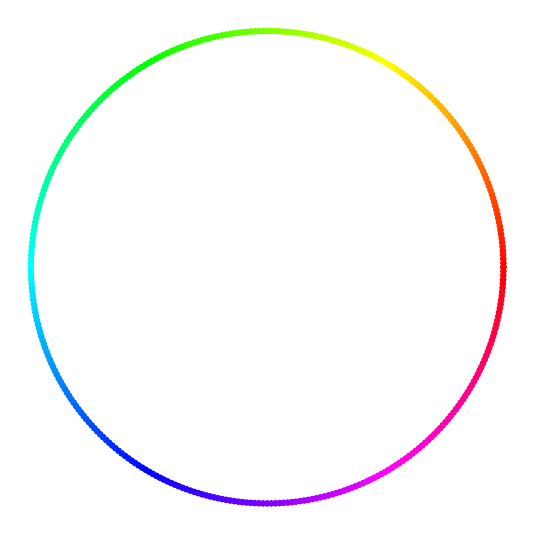
\begin{tikzpicture}
	\foreach \thetawheel in {0,1,...,360}
	{
		%\tdplotcalcrgb{\thetawheel}
		\pgfmathdivide{\thetawheel}{360}
		\definecolor{tdplotcolor}{hsb}{\pgfmathresult, 1, 1}
		\color{tdplotcolor}
		\filldraw(\thetawheel:3) circle (1pt);
	}
\end{tikzpicture}
}



\newcommand{\tikzname}{Ti\emph{k}Z}
\newcommand{\tdplot}{\texttt{tikz-3dplot}}


\title{The \texttt{\tdplot} Package}

\author{Jeff Hein\\ \url{http://tikz3dplot.wordpress.com}}




\newcommand{\tdplotlocation}{\url{http://www.ctan.org}}

\settocdepth{subsection}

\setsecnumdepth{subsection}
\maxsecnumdepth{subsection}
\settocdepth{subsection}
\maxtocdepth{subsection}


\newif\ifscratch		%for doing scratchpad work, this cuts out the rest of the document


%**************** Example Box *********************

\definecolor{shadecolor}{rgb}{0.90,0.90,0.90}
%this defines an environment for presenting code in an indented, shaded, verbatim, multipage region.  Requires framed, alltt, and color environments, and \definecolor{shadecolor}{rgb}{0.90,0.90,0.90}

%this sets the verbatim font and size, based on the memoir class usage
\setverbatimfont{\normalfont\ttfamily\footnotesize}
%this turns tabs on in the verbatim environment
\tabson[4]
%this sets the frequency of line numbers displayed in a boxedverbatim environment
%\linenumberfrequency{1}
%this sets the font size of line numbers in a boxedverbatim environment
\linenumberfont{\normalfont\ttfamily\tiny}
%this positions line numbers outside the box of a boxedverbatim environment
%\bvnumbersoutside
%this turns off the box of a boxedverbatim environment
\nobvbox


\begin{document}

\input{Scratchpad.tex}



\ifscratch
	\end{document}
\fi


\frontmatter
\pagestyle{empty}

\maketitle



\begin{figure}[h]
	\begin{center}
	\tdplotmainfig
	\threedsurfaceplot

	\threedalphabetagamma
	%A 3d coordinate system rendered in \tikzname using the \tdplot\ package.  The user can specify the display perspective by specifying angles $\theta_d$ and $\phi_d$, which rotate the coordinate frame from the ``standard'' display position where $x$ points to the right, $y$ points up.
	\end{center}
\end{figure}

\cleardoublepage

{

	\input{ tikz-3dplot_changelog.tex }

	\vfill
  \parindent=0pt
  Copyright 2010-2012 Jeff Hein

	\medskip
  Permission is granted to distribute and/or modify \emph{both
  the documentation and the code} under the conditions of the LaTeX
  Project Public License, either version 1.3 of this license or (at
  your option) any later version.  The latest version of this license is in
  http://www.latex-project.org/lppl.txt
	
	\clearpage
}

\pagenumbering{roman}
\tableofcontents
\cleardoublepage
\pagenumbering{arabic}

\mainmatter

\pagestyle{plain}

\chapter{Introduction}\label{cha:intro}

\section{Overview of the \tdplot\ Package}
The \tdplot\ package offers commands and coordinate transformation styles for \tikzname, providing relatively straightforward tools to draw three-dimensional coordinate systems and simple three-dimensional diagrams.  The package is currently in its infancy, and is subject to change.  Comments or suggestions are encouraged.

This document describes the basics of the \tdplot\ package and provides information about the various available commands.  Examples are given where possible.

\subsection{What \tdplot\ is}

\tdplot\ provides commands to easily specify coordinate transformations for \tikzname, allowing for relatively easy plotting.  I needed to draw accurate 3d vector images for a physics thesis, and this package was developed to meet this need.

Various plotting commands are used to identify coordinate locations using spherical polar or Cartesian coordinates.  Coordinate transformation commands allow for the calculation of a coordinate in one frame based on its values in another frame.  Some drawing commands have been developed to assist in the rendering of arcs.  These commands do the number crunching required to position and render the arcs.  These commands are discussed in Section \ref{sec:tdplotcommands}. 

In addition, the \verb|\tdplotsphericalsurfaceplot| was developed to render three-dimensional surfaces in spherical polar coordinates, where the radius is expressed in terms of a user-defined function of $\theta$ and $\phi$.  With this function, the surface hue can be given explicitly, or expressed as a user-defined function of $r$, $\theta$, and $\phi$.  This command is discussed in Section \ref{sec:spherical_surface_plot}.

\begin{figure}[ht]
	\begin{center}
		\threedconventions
	\end{center}
	\caption{\tdplot\ coordinate and positive angle convention.}\label{fig:conventions}
\end{figure}

In \tdplot, a right-handed coordinate system convention is used.  In addition, all positive angles  constitute a right-hand screw sense of rotation (see Figure \ref{fig:conventions}).  This means that a positive rotation about a given axis refers to a clockwise rotation when viewing along the direction the axis, or counterclockwise when viewing against the direction of the axis.

\subsection{What \tdplot\ is not}

\tdplot\ does not, in general, consider polygons, surfaces, or object opacity.  The one exception is the \verb|\tdplotsphericalsurfaceplot| command, specifically designed to render spherical polar surfaces.  The \verb|\tdplotsphericalsurfaceplot| command is discussed in Section \ref{sec:spherical_surface_plot}.

Tools like Sketch by Gene Ressler are better suited for more rigorous surface rendering.  These can be found at \url{http://www.frontiernet.net/~eugene.ressler/}

\subsection{Similar Work}

To my knowledge, there is no other package available which allows straightforward rendering of 3d coordinates in \tikzname, directly in a \LaTeX\ document.  Since this project is in its infancy, this may be subject to change based on feedback.

\subsubsection{Sketch}

The Sketch project can provide three-dimensional rendering of axes, points, and lines, but (as far as I understand the program) cannot draw arcs without using a series of line segments.  Further, Sketch requires an external program to render the image, while \tdplot\ can be developed and maintained right in a \LaTeX\ document.

\subsubsection{\TeX ample.net}

There are a variety of \tikzname\ examples listed at \url{http://www.texample.net/tikz/examples}.  Some of these examples gave me inspiration to make this package.  Some examples of note include the following:

\begin{itemize}
	\item 3D cone
		\begin{description}
			\item[Author:] Eugene Ressler
			\item[url:] \url{http://www.texample.net/tikz/examples/3d-cone/}
			\item[Notes:] This demonstrates the use of Sketch in TikZ figures.
		\end{description}
	\item Annotated 3D box
		\begin{description}
			\item[Author] Alain Matthes
			\item[url] \url{http://www.texample.net/tikz/examples/annotated-3d-box/}
			\item[Notes] This example demonstrates the direct use of coordinate transformations, as well as performing math directly within coordinates.
		\end{description}
	\item Cluster of atoms
		\begin{description}
			\item[Author] Agustin E. Bolzan
			\item[url] \url{http://www.texample.net/tikz/examples/clusters-of-atoms/}
			\item[Notes] This uses shifts and slants rather than rotations to render an isometric look.
		\end{description}
	\item Plane partition
		\begin{description}
			\item[Author] Jang Soo Kim
			\item[url] \url{http://www.texample.net/tikz/examples/plane-partition/}
			\item[Notes] This example draws solid surfaces with coordinate axes defined by rotations around the \tikzname\ standard coordinate frame.
		\end{description}
	\item Spherical and cartesian grids
		\begin{description}
			\item[Author] Marco Miani
			\item[url] \url{http://www.texample.net/tikz/examples/spherical-and-cartesian-grids/}
			\item[Notes] This example renders arcs and lines in three dimensions using explicit calculations.  It takes into account the opacity of the spherical example, by showing hidden lines behind the sphere as dashed lines.
		\end{description}
	\item Stereographic and cylindrical map projections
		\begin{description}
			\item[Author] Thomas M. Trzeciak
			\item[url] \url{http://www.texample.net/tikz/examples/map-projections/}
			\item[Notes] This example illustrates the use of coordinate transformations to draw planes and arcs for spherical coordinates.
		\end{description}
\end{itemize}


\section{Installing the \tdplot\ Package}

Get a copy of \tdplot\ from \tdplotlocation.  Place the style file in the same directory as your \LaTeX\ project.  In your preamble, add the following line:
%
\begin{shaded}
\begin{verbatim}
\usepackage{tikz-3dplot}
\end{verbatim}
\end{shaded}

Make sure this line is written after all other required packages.


\subsection{\tdplot\ Requirements}

To use this package, the following other packages must be loaded in the preamble first:
\begin{itemize}
\item \tikzname
\item \texttt{ifthen} (for the \texttt{tdplotsphericalsurfaceplot} command)
\end{itemize} 


\subsection{\tdplot\ Package Options}

Currently there are no options available for the \tdplot\ package.

\section{Using the \tdplot\ Package}

\tdplot\ provides styles and commands which are useful in a \texttt{tikzpicture} environment.  These commands and styles are described in Chapter \ref{cha:using_tdplot}.









\chapter{Overview of 3d in \tdplot}\label{cha:overview3d}

\section{\tikzname\ 3d Plotting} \label{sec:tikzplotting}

When setting up a tikzpicture or a drawing style, the $x$, $y$, and $z$ axes can be specified directly in terms of the original coordinate system.  The following example shows how a \texttt{tikzpicture} environment can be configured to use customized axes.

\begin{shaded}
\begin{verbatim}
\begin{tikzpicture}[%
	x={(\raarot cm,\rbarot cm)},%
	y={(\rabrot cm, \rbbrot cm)},%
	z={(\racrot, \rbcrot cm)}]
\end{verbatim}
\end{shaded}

In this example, the terms \verb|\raarot| and so on specify how the coordinates are represented in the original \tikzname\ coordinate system, and are calculated by the \tdplot\ package.  Note that units are explicitly required so \tikzname\ understands that these are absolute coordinates, not scales on the existing axis.  See the PGF manual Version 2.00, section 21.2 on pages 217-218 for details on \tikzname\ coordinate transformations.

\section{The \tdplot\ Main Coordinate System}\label{sec:main_theory}

\tdplot\ offers two coordinate systems, namely the \emph{main} coordinate system $(x,y,z)$, and the \emph{rotated} coordinate system $(x',y',z')$.  The latter system is described in Section \ref{sec:rotated_theory}.

As the name suggests, the main coordinate system provides a user-specified transformation to render 3d points in a \texttt{tikzpicture} environment. The orientation of the main coordinate system is defined by the angles $\theta_{d}$ and $\phi_{d}$.  In the unrotated ($\theta_{d} = \phi_{d} = 0$) position, the $xy$ plane of the main coordinate system coincides with the default orientation for a \texttt{tikzpicture} environment, while $z$ points ``out of the page''.
%
The coordinate system is positioned by the following operations:
%
\begin{itemize}
	\item Rotate the coordinate system about the body $x$ axis by the amount $\theta_d$, and
	\item Rotate the coordinate system about the (rotated) body $z$ axis by the amount $\phi_d$.
\end{itemize}

In this rotation sense, the $z$ axis will always point in the vertical page direction.  This transformation is given  by the rotation matrix $R_d(\theta_d,\phi_d)$, as
%
\begin{align}\begin{split}
	R^d(\theta_d,\phi_d) &= R^{z'}(\phi_d)R^{x}(\theta_d)\\
		&= \begin{pmatrix}
			\cos\phi_d & -\sin\phi_d & 0\\
			\sin\phi_d & \cos\phi_d & 0\\
			0 & 0 & 1
		\end{pmatrix}
		\begin{pmatrix}
			1 & 0 & 0\\
			0 & \cos\theta_d & -\sin\theta_d\\
			0 & \sin\theta_d & \cos\theta_d\\
		\end{pmatrix}\\
		&= \begin{pmatrix}
			\cos\phi_d & \sin\phi_d & 0\\
			-\cos\theta_d\sin\phi_d & \cos\theta_d\cos\phi_d & -\sin\theta_d\\
			\sin\theta_d\sin\phi_d & -\sin\theta_d\cos\phi_d & \cos\theta_d\\
		\end{pmatrix}
\end{split}\end{align}

\begin{figure}[b]
	\begin{center}
		\threedcoord{0}{0}
		\threedcoord{10}{50}
		\threedcoord{30}{110}
	
		\threedcoord{40}{150}
		\threedcoord{60}{170}
		\threedcoord{90}{180}
	\end{center}
	\caption{Examples of coordinate systems for various choices of $\theta_d$ and $\phi_d$.}
\end{figure}

Using this matrix, the \tikzname\ coordinate transformation can be applied as described in Section \ref{sec:tikzplotting} by the various matrix elements, as
%
\begin{align}\begin{split}
	x &= (R^d_{1,1}, R^d_{2,1})\\
	y &= (R^d_{1,2}, R^d_{2,2})\\
	z &= (R^d_{1,3}, R^d_{2,3})
\end{split}\end{align}

Note that the third row of the rotation matrix is not needed for this transformation, since a screen coordinate is a 2d value.  Once the transformed axes have been established, any 3d coordinate specified in \tikzname\ will adhere to the transformation, yielding a 3D representation.  Lines and nodes can readily be drawn by using these 3d coordinates.  

This coordinate transformation is accessible through \tdplot\ using the command \texttt{tdplotsetmaincoords}, as described in Chapter \ref{cha:using_tdplot}.

\section{The \tdplot\ Rotated Coordinate System}\label{sec:rotated_theory}

Along with the main coordinate system, described in Section \ref{sec:main_theory}, \tdplot\ offers a \emph{rotated} coordinate system that is defined with respect to the main coordinate system.  This system can be rotated to any position using Euler rotations, and can be translated so the origin of the rotated coordinate system sits on an arbitrary point in the main coordinate system.

Three rotations can be performed to give any arbitrary orientation of a rotated coordinate system.  By convention, the following rotations are chosen:
%
\begin{itemize}
	\item Rotate by angle $\gamma$ about the world $z$ axis,
	\item Rotate by angle $\beta$ about the (unrotated) world $y$ axis, and
	\item Rotate by angle $\alpha$ about the (unrotated) world $z$ axis.
\end{itemize}

These rotations are shown in Figure \ref{fig:euler_angles}.

\begin{figure}[h]
	\begin{center}
		\threedalphabetagamma
	\end{center}
	\caption{Positioning the rotated coordinate frame $(x', y', z')$ using Euler angles $(\alpha, \beta, \gamma)$.}\label{fig:euler_angles}
\end{figure}


This rotation matrix $D(\alpha,\beta,\gamma)$ is given by
%
\begin{align}\begin{split}
	D(\alpha,\beta,\gamma) &= R^z(\alpha)R^y(\beta)R^z(\gamma)\\
	&= \begin{pmatrix}
			\cos\alpha & -\sin\alpha & 0\\
			\sin\alpha & \cos\alpha & 0\\
			0 & 0 & 1\\
		\end{pmatrix}
		\begin{pmatrix}
			\cos\beta & 0 & \sin\beta \\
			0 & 1 & 0 \\
			-\sin\beta & 0 & \cos\beta\\
		\end{pmatrix}
		\begin{pmatrix}
			\cos\gamma & -\sin\gamma & 0\\
			\sin\gamma & \cos\gamma & 0\\
			0 & 0 & 1\\
		\end{pmatrix}\\
	&= \begin{pmatrix}
		\cos\alpha\cos\beta\cos\gamma - \sin\alpha\sin\gamma & -\cos\alpha\cos\beta\sin\gamma - \sin\alpha\cos\gamma & \cos\alpha\sin\beta\\
		\sin\alpha\cos\beta\cos\gamma + \cos\alpha\sin\gamma & -\sin\alpha\cos\beta\sin\gamma + \cos\alpha\cos\gamma & \sin\alpha\sin\beta\\
		-\sin\beta\cos\gamma & \sin\beta\sin\gamma & \cos\beta
		\end{pmatrix}
\end{split}\end{align}

To define the rotated coordinate frame, this rotation matrix is applied after rotation matrix $R^d(\theta_d,\phi_d)$ used to define the main coordinate frame.  The full transformation for the rotated coordinate frame is then given by 
%
\begin{align}
	R'^d(\theta_d,\phi_d,\alpha,\beta,\gamma) &= D(\alpha,\beta,\gamma)R^d(\theta_d,\phi_d)
\end{align}

Using this matrix, the \tikzname\ coordinate transformation can be applied as described in Section \ref{sec:tikzplotting} by the various matrix elements, as
%
\begin{align}\begin{split}
	x' &= (R'^d_{1,1}, R'^d_{2,1})\\
	y' &= (R'^d_{1,2}, R'^d_{2,2})\\
	z' &= (R'^d_{1,3}, R'^d_{2,3})
\end{split}\end{align}

This coordinate transformation is accessible through \tdplot\ using the command \texttt{tdplotsetrotatedcoords}, as described in Chapter \ref{cha:using_tdplot}.

\begin{figure}[h]
	\begin{center}
		\threedrotcoordsystem
	\end{center}
	\caption{The rotated coordinate frame $(x', y', z')$ displayed within the main coordinate frame $(x,y,z)$.  Both are completely specified by user-defined angles: $(\theta_d, \phi_d)$ for the main coordinate frame, and $(\alpha, \beta, \gamma)$ for the rotated coordinate frame.}
\end{figure}


\section{Arcs in 3d, and the ``Theta Plane''}

Arcs can be drawn in \tikzname\ using commands described in the PGF manual Version 2.00, section 2.10 on pages 25-26.  However, the arc commands accept 2d coordinates, and thus can only be drawn in the $xy$ plane.  

To draw an arc in any position other than within the $xy$ plane of the main coordinate frame, the rotated coordinate frame must be used, where the $x'y'$ plane lies in the desired orientation within the main coordinate frame.  Such an arc is needed, for example, when illustrating the polar angle $\theta$ of some vector.  This $\theta$ arc exists in a plane which contains the $z$ axis, and is rotated about the $z$ axis by the angle $\phi$ from the $xz$ plane.  For lack of a better name, this plane is referred to as the ``theta plane'' within a given coordinate system.

\begin{figure}[h]
	\begin{center}
	\threedthetaarc
	\end{center}
	\caption{Drawing arcs outside the $xy$ plane by using a rotated coordinate frame in the ``theta plane'' of the main coordinate frame.}
\end{figure}

As described in Chapter \ref{cha:using_tdplot}, \tdplot\ offers the commands \texttt{tdplotsetthetaplanecoords} and \texttt{tdplotsetrotatedthetaplanecoords} to easily configure the rotated coordinate frame to lie within the desired theta plane.








\chapter{Using the \tdplot\ Package} \label{cha:using_tdplot}

The \tdplot\ package was developed to handle the number crunching described in Chapter \ref{cha:overview3d}, and provide a relatively simple and straightforward front-end for users.  

The main and rotated coordinate frames are configured by using commands described in Section \ref{sec:tdplotcommands}.  These commands generate \tikzname\ styles which can be used either in defining the \texttt{tikzpicture} environment, or directly in any \tikzname\ command.  The styles are described further in Section \ref{sec:tikzstyles}.

\section{The \tdplot\ \tikzname\ Styles} \label{sec:tikzstyles}


\subsection{\texttt{tdplot\_main\_coords}}

The \verb|tdplot_main_coords| style stores the coordinate transformation required to generate the main coordinate system.  This style can either be used when the \texttt{tikzpicture} environment is started, or when an individual \tikzname\ plotting command is used.

\subsection{\texttt{tdplot\_rotated\_coords}}

The \verb|tdplot_rotated_coords| style stores the coordinate transformation (translation and rotation) required to generate the rotated coordinate system within the main coordinate system.  This style can either be used when the \texttt{tikzpicture} environment is started, or when an individual \tikzname\ plotting command is used.

\subsection{\texttt{tdplot\_screen\_coords}}

The \verb|tdplot_screen_coords| style provides the standard, unrotated \tikzname\ coordinate frame.  This is useful to escape out of the user-defined 3d coordinates used at the beginning of the \texttt{tikzpicture} environment, and place something on an absolute scale in the figure.  Tables, legends, and captions contained within the same figure as a 3d plot can make use of this style.

%\section{The \tdplot\ Macros} \label{sec:tdplotmacros}
%
%\tdplot\ uses various macros to perform all its number crunching.  Some of these are only used ``under the hood'', where the user would never need to know about them, while others are required to pass numbers to, or receive results from, the \tdplot\ commands.
%
%Since my knowledge of LaTeX is limited, there is probably a more streamlined and efficient way I can handle all this.  As such, feedback and suggestions are welcome.
%
%\subsection{``Input'' Macros}
%
%These macros must be defined by the user before calling the corresponding command.  In some cases, they are defined explicitly by another command, as described in the following section.
%
%\begin{center}
%	\begin{tabular}{c p{4in}}
%		\hline
%		\textbf{Macro} & \textbf{Notes}\\
%		\hline
%		
%		\hline
%	\end{tabular}
%\end{center}
%
%\subsection{''Output'' Macros}
%
%These macros are defined as a result of calling a command.  These can either be used directly by the user, or by subsequent \tdplot\ commands.
%
%\begin{center}
%	\begin{tabular}{c p{4in}}
%		\hline
%		\textbf{Macro} & \textbf{Notes}\\
%		\hline
%		\verb|\tdplotresx| & Result x value
%		
%		\hline
%	\end{tabular}
%\end{center}
%
%\subsection{``Under the Hood'' Macros}
%
%These are macros which are not necessary to know about.  They are used so \tdplot\ can perform its task, and are not used outside the commands.
%
%\begin{center}
%	\begin{tabular}{c p{4in}}
%		\hline
%		\textbf{Macro} & \textbf{Notes}\\
%		\hline
%			\verb|\lowerphi| & Lower $\phi$ limit for \verb|\tdplotsphericalsurfaceplot| polar plot.\\
%			\verb|\upperphi| & Upper $\phi$ limit for \verb|\tdplotsphericalsurfaceplot| polar plot.\\
%			\verb|\lowertheta| & Lower $\theta$ limit for \verb|\tdplotsphericalsurfaceplot| polar plot.\\
%			\verb|\uppertheta| & Upper $\theta$ limit for \verb|\tdplotsphericalsurfaceplot| polar plot.\\
%		\hline
%	\end{tabular}
%\end{center}

\section{The \tdplot\ Commands} \label{sec:tdplotcommands}

This section lists the various commands provided by the \tdplot\ package.  Examples are provided where it is useful.

\section{Coordinate Configuration Commands}

\subsection{\texttt{tdplotsetmaincoords}}

\begin{description}
	\item[Description:] Generates the style \verb|tdplot_main_coords| which provides the coordinate transformation for the main coordinate frame, based on a user-specified orientation $(\theta_d,\phi_d)$.  $\theta_d$ denotes the rotation around the $x$ axis, while $\phi_d$ denotes the rotation around the $z$ axis. Note that $(0,0)$ is the default orientation, where $x$ points right, $y$ points up, and $z$ points ``out of the page''.

	\item[Syntax:] \verb|\tdplotsetmaincoords{| $\theta_d$ \verb|}{| $\phi_d$ \verb|}|

	\item[Parameters:]~
		\begin{description}
			\item[$\theta_d$] The angle (in degrees) through which the coordinate frame is rotated about the $x$ axis.
			\item[$\phi_d$] The angle (in degrees) through which the coordinate frame is rotated about the $z$ axis.
		\end{description}
	\item[Example:] ~
\begin{shaded}
\begin{verbatim}
\tdplotsetmaincoords{70}{110}
\begin{tikzpicture}[tdplot_main_coords]
	\draw[thick,->] (0,0,0) -- (1,0,0) node[anchor=north east]{$x$};
	\draw[thick,->] (0,0,0) -- (0,1,0) node[anchor=north west]{$y$};
	\draw[thick,->] (0,0,0) -- (0,0,1) node[anchor=south]{$z$};
\end{tikzpicture}
\end{verbatim}
\tdplotsetmaincoords{70}{110}
\begin{tikzpicture}[tdplot_main_coords]
	\draw[thick,->] (0,0,0) -- (1,0,0) node[anchor=north east]{$x$};
	\draw[thick,->] (0,0,0) -- (0,1,0) node[anchor=north west]{$y$};
	\draw[thick,->] (0,0,0) -- (0,0,1) node[anchor=south]{$z$};
\end{tikzpicture}
\end{shaded}

\end{description}

\subsection{\texttt{tdplotsetrotatedcoords}}

\begin{description}
	\item[Description:] Generates the style \verb|tdplot_rotated_coords| which provides the coordinate transformation for rotated coordinate frame within the current main coordinate frame, based on user-specified Euler angles $(\alpha,\beta,\gamma)$.  Rotations use the $z(\alpha)y(\beta)z(\gamma)$ convention of Euler rotations, where the system is rotated by $\gamma$ about the $z$ axis, then $\beta$ about the (world) $y$ axis, and then $\alpha$ about the (world) $z$ axis.
	\item[Syntax:] \verb|\tdplotsetrotatedcoords{|$\alpha$\verb|}{|$\beta$\verb|}{|$\gamma$\verb|}|
	\item[Parameters:]~
		\begin{description}
			\item[$\alpha$] The angle (in degrees) through which the rotated frame is rotated about the world $z$ axis.
			\item[$\beta$] The angle (in degrees) through which the rotated frame is rotated about the world $y$ axis.
			\item[$\gamma$] The angle (in degrees) through which the rotated frame is rotated about the world $z$ axis.
		\end{description}
	\item[Example:] ~
\begin{shaded}
\begin{verbatim}
\tdplotsetmaincoords{70}{110}
\begin{tikzpicture}[tdplot_main_coords]
	\draw[thick,->] (0,0,0) -- (1,0,0) node[anchor=north east]{$x$};
	\draw[thick,->] (0,0,0) -- (0,1,0) node[anchor=north west]{$y$};
	\draw[thick,->] (0,0,0) -- (0,0,1) node[anchor=south]{$z$};

	\tdplotsetrotatedcoords{60}{40}{30}

	\draw[thick,color=blue,tdplot_rotated_coords,->] (0,0,0) --
		(.7,0,0) node[anchor=north]{$x'$};
	\draw[thick,color=blue,tdplot_rotated_coords,->] (0,0,0) --
		(0,.7,0) node[anchor=west]{$y'$};
	\draw[thick,color=blue,tdplot_rotated_coords,->] (0,0,0) --
		(0,0,.7) node[anchor=south]{$z'$};
\end{tikzpicture}
\end{verbatim}
\tdplotsetmaincoords{70}{110}
\begin{tikzpicture}[tdplot_main_coords]
	\draw[thick,->] (0,0,0) -- (1,0,0) node[anchor=north east]{$x$};
	\draw[thick,->] (0,0,0) -- (0,1,0) node[anchor=north west]{$y$};
	\draw[thick,->] (0,0,0) -- (0,0,1) node[anchor=south]{$z$};

	\tdplotsetrotatedcoords{60}{40}{30}

	\draw[thick,color=blue,tdplot_rotated_coords,->] (0,0,0) -- (.7,0,0) node[anchor=north]{$x'$};
	\draw[thick,color=blue,tdplot_rotated_coords,->] (0,0,0) -- (0,.7,0) node[anchor=west]{$y'$};
	\draw[thick,color=blue,tdplot_rotated_coords,->] (0,0,0) -- (0,0,.7) node[anchor=south]{$z'$};
\end{tikzpicture}
\end{shaded}
\end{description}


\subsection{\texttt{tdplotsetrotatedcoordsorigin}}

\begin{description}
	\item[Description:]  Sets the origin of the rotated coordinate system specified by \verb|tdplot_rotated_coords| using a user-defined point.  This point can be either a literal or predefined point.
	\item[Syntax:] \verb|\tdplotsetrotatedcoordsorigin{point}|
	\item[Parameters:]~
		\begin{description}
			\item[\texttt{point}] A point predefined using the \tikzname\ \verb|\coordinate| command.
		\end{description}
	\item[Example:] ~
\begin{shaded}
\begin{verbatim}
\tdplotsetmaincoords{70}{110}
\begin{tikzpicture}[tdplot_main_coords]
	\draw[thick,->] (0,0,0) -- (1,0,0) node[anchor=north east]{$x$};
	\draw[thick,->] (0,0,0) -- (0,1,0) node[anchor=north west]{$y$};
	\draw[thick,->] (0,0,0) -- (0,0,1) node[anchor=south]{$z$};

	\tdplotsetrotatedcoords{60}{40}{30}

	\coordinate (Shift) at (0.5,0.5,0.5);
	\tdplotsetrotatedcoordsorigin{(Shift)}

	\draw[thick,color=blue,tdplot_rotated_coords,->] (0,0,0) --
		(.7,0,0) node[anchor=north]{$x'$};
	\draw[thick,color=blue,tdplot_rotated_coords,->] (0,0,0) --
		(0,.7,0) node[anchor=west]{$y'$};
	\draw[thick,color=blue,tdplot_rotated_coords,->] (0,0,0) --
		(0,0,.7) node[anchor=south]{$z'$};
\end{tikzpicture}
\end{verbatim}
\tdplotsetmaincoords{70}{110}
\begin{tikzpicture}[tdplot_main_coords]
	\draw[thick,->] (0,0,0) -- (1,0,0) node[anchor=north east]{$x$};
	\draw[thick,->] (0,0,0) -- (0,1,0) node[anchor=north west]{$y$};
	\draw[thick,->] (0,0,0) -- (0,0,1) node[anchor=south]{$z$};

	\tdplotsetrotatedcoords{60}{40}{30}

	\coordinate (Shift) at (0.5,0.5,0.5);
	\tdplotsetrotatedcoordsorigin{(Shift)}

	\draw[thick,color=blue,tdplot_rotated_coords,->] (0,0,0) -- (.7,0,0) node[anchor=north]{$x'$};
	\draw[thick,color=blue,tdplot_rotated_coords,->] (0,0,0) -- (0,.7,0) node[anchor=west]{$y'$};
	\draw[thick,color=blue,tdplot_rotated_coords,->] (0,0,0) -- (0,0,.7) node[anchor=south]{$z'$};
\end{tikzpicture}
\end{shaded}
\end{description}

\subsection{\texttt{tdplotresetrotatedcoordsorigin}}

\begin{description}
	\item[Description:] Resets the origin of the rotated coordinate system back to the origin of the main coordinate system.
	\item[Syntax:] \verb|\tdplotresetrotatedcoordsorigin|
	\item[Parameters:] None
\end{description}

\subsection{\texttt{tdplotsetthetaplanecoords}}

\begin{description}
	\item[Description:] Generates a rotated coordinate system such that the $x'y'$ plane is coplanar to a plane containing the polar angle $\theta$ projecting from the main coordinate system $z$ axis.  This coordinate system is particularly useful for drawing within this ``theta plane'', as \tikzname\ draws arcs in the $xy$ plane.  As with \texttt{tdplotsetrotatedcoords}, this coordinate system is accessible through the \verb|tdplot_rotated_coords| style.  Note that any rotated coordinate frame offset previously set by \texttt{tdplotsetrotatedcoordsorigin} is automatically reset when this command is used.
	\item[Syntax:] \verb|\tdplotsetthetaplanecoords{|$\phi$\verb|}|
	\item[Parameters:]~
		\begin{description}
			\item[$\phi$] The angle (in degrees) through which the ``theta plane'' makes with the $xz$ plane of the main coordinate system.
		\end{description}
	\item[Example:]~
\begin{shaded}
\begin{verbatim}
\tdplotsetmaincoords{70}{110}

\begin{tikzpicture}[scale=3,tdplot_main_coords]
	\draw[thick,->] (0,0,0) -- (1,0,0) node[anchor=north east]{$x$};
	\draw[thick,->] (0,0,0) -- (0,1,0) node[anchor=north west]{$y$};
	\draw[thick,->] (0,0,0) -- (0,0,1) node[anchor=south]{$z$};

	\tdplotsetcoord{P}{.8}{50}{70}

	%draw a vector from origin to point (P) 
	\draw[-stealth,color=red] (O) -- (P);

	%draw projection on xy plane, and a connecting line
	\draw[dashed, color=red] (O) -- (Pxy);
	\draw[dashed, color=red] (P) -- (Pxy);


	\tdplotsetthetaplanecoords{70}

	\draw[tdplot_rotated_coords,color=blue,thick,->] (0,0,0)
		-- (.2,0,0) node[anchor=east]{$x'$};
	\draw[tdplot_rotated_coords,color=blue,thick,->] (0,0,0)
		-- (0,.2,0) node[anchor=north]{$y'$};
	\draw[tdplot_rotated_coords,color=blue,thick,->] (0,0,0)
		-- (0,0,.2) node[anchor=west]{$z'$};

\end{tikzpicture}
\end{verbatim}
\tdplotsetmaincoords{70}{110}

\begin{tikzpicture}[scale=3,tdplot_main_coords]
	\draw[thick,->] (0,0,0) -- (1,0,0) node[anchor=north east]{$x$};
	\draw[thick,->] (0,0,0) -- (0,1,0) node[anchor=north west]{$y$};
	\draw[thick,->] (0,0,0) -- (0,0,1) node[anchor=south]{$z$};

	\tdplotsetcoord{P}{.8}{50}{70}

	\coordinate (O) at (0,0,0);

	%draw a vector from origin to point (P) 
	\draw[-stealth,color=red] (O) -- (P);

	%draw projection on xy plane, and a connecting line
	\draw[dashed, color=red] (O) -- (Pxy);
	\draw[dashed, color=red] (P) -- (Pxy);

	\tdplotsetthetaplanecoords{70}

	\draw[tdplot_rotated_coords,color=blue,thick,->] (0,0,0)
		-- (.2,0,0) node[anchor=east]{$x'$};
	\draw[tdplot_rotated_coords,color=blue,thick,->] (0,0,0)
		-- (0,.2,0) node[anchor=north]{$y'$};
	\draw[tdplot_rotated_coords,color=blue,thick,->] (0,0,0)
		-- (0,0,.2) node[anchor=west]{$z'$};

\end{tikzpicture}
\end{shaded}
\end{description}


\subsection{\texttt{tdplotsetrotatedthetaplanecoords}}

\begin{description}
	\item[Description:] Just like \texttt{tdplotsetthetaplanecoords}, except this works for the rotated coordinate system.  Generates a rotated coordinate system such that the $x'-y'$ plane is coplanar to a plane containing the polar angle $\theta'$ projecting from the current rotated coordinate system $z'$ axis.  Note that the current rotated coordinate system is overwritten by this theta plane coordinate system after the command is completed.
	\item[Syntax:] \verb|\tdplotsetrotatedthetaplanecoords{|$\phi'$\verb|}|
	\item[Parameters:]~
		\begin{description}
			\item[$\phi'$] The angle (in degrees) through which the ``theta plane'' makes with the $x'-z'$ plane of the current rotated coordinate system.
		\end{description}
	\item[Example:]~
\begin{shaded}
\begin{verbatim}
\tdplotsetmaincoords{60}{110}
\begin{tikzpicture}[scale=3,tdplot_main_coords]
	\draw[thick,->] (0,0,0) -- (1,0,0) node[anchor=north east]{$x$};
	\draw[thick,->] (0,0,0) -- (0,1,0) node[anchor=north west]{$y$};
	\draw[thick,->] (0,0,0) -- (0,0,1) node[anchor=south]{$z$};

	\coordinate (Shift) at (2,2,2);

	\tdplotsetrotatedcoords{-20}{10}{0}
	\tdplotsetrotatedcoordsorigin{(Shift)}

	\draw[thick,color=blue,tdplot_rotated_coords,->] (0,0,0)
		-- (1,0,0) node[anchor=south east]{$x'$};
	\draw[thick,color=blue,tdplot_rotated_coords,->] (0,0,0)
		-- (0,1,0) node[anchor=west]{$y'$};
	\draw[thick,color=blue,tdplot_rotated_coords,->] (0,0,0)
		-- (0,0,1) node[anchor=south]{$z'$};

	\tdplotsetrotatedthetaplanecoords{30}

	\draw[thick,color=blue,tdplot_rotated_coords,->] (0,0,0)
		-- (.5,0,0) node[anchor=south east]{$x''$};
	\draw[thick,color=blue,tdplot_rotated_coords,->] (0,0,0)
		-- (0,.5,0) node[anchor=west]{$y''$};
	\draw[thick,color=blue,tdplot_rotated_coords,->] (0,0,0)
		-- (0,0,.5) node[anchor=south]{$z''$};
\end{tikzpicture}
\end{verbatim}
\ifpdf
\tdplotsetmaincoords{60}{110}
\begin{tikzpicture}[scale=3,tdplot_main_coords]
	\draw[thick,->] (0,0,0) -- (1,0,0) node[anchor=north east]{$x$};
	\draw[thick,->] (0,0,0) -- (0,1,0) node[anchor=north west]{$y$};
	\draw[thick,->] (0,0,0) -- (0,0,1) node[anchor=south]{$z$};

	\coordinate (Shift) at (2,2,2);

	\tdplotsetrotatedcoords{-20}{10}{0}
	\tdplotsetrotatedcoordsorigin{(Shift)}

	\draw[thick,color=blue,tdplot_rotated_coords,->] (0,0,0) -- (1,0,0) node[anchor=south east]{$x'$};
	\draw[thick,color=blue,tdplot_rotated_coords,->] (0,0,0) -- (0,1,0) node[anchor=west]{$y'$};
	\draw[thick,color=blue,tdplot_rotated_coords,->] (0,0,0) -- (0,0,1) node[anchor=south]{$z'$};

	\tdplotsetrotatedthetaplanecoords{30}

	\draw[thick,color=blue,tdplot_rotated_coords,->] (0,0,0) -- (.5,0,0) node[anchor=south east]{$x''$};
	\draw[thick,color=blue,tdplot_rotated_coords,->] (0,0,0) -- (0,.5,0) node[anchor=west]{$y''$};
	\draw[thick,color=blue,tdplot_rotated_coords,->] (0,0,0) -- (0,0,.5) node[anchor=south]{$z''$};
\end{tikzpicture}
\fi
\end{shaded}

\end{description}

\subsection{\texttt{tdplotcalctransformmainrot}}

\begin{description}
	\item[Description:]  Calculates the rotation matrix used to transform a coordinate from the main coordinate frame to the rotated coordinate frame.  The matrix elements are stored in the macros \verb|\raaeul| through \verb|\rcceul|.  This transformation is accessed using \verb|\tdplottransformmainrot|.
\end{description}


\subsection{\texttt{tdplotcalctransformrotmain}}

\begin{description}
	\item[Description:]  Calculates the rotation matrix used to define the rotated coordinate frame, as well as transform a coordinate from the rotated coordinate frame to the main coordinate frame.  The matrix elements are stored in the macros \verb|\raaeul| through \verb|\rcceul|.  This transformation is used in the \verb|\tdplotsetrotatedcoords| command, and is accessed using \verb|\tdplottransformrotmain|.
\end{description}

\subsection{\texttt{tdplotcalctransformmainscreen}}

\begin{description}
	\item[Description:]  Calculates the rotation matrix used to define the main coordinate frame, as well as transform a coordinate from the main coordinate frame to the screen coordinate frame.  The matrix elements are stored in the macros \verb|\raarot| through \verb|\rccrot|.  This transformation is used in the \verb|\tdplotsetmaincoords| command, and is accessed using \verb|\tdplottransformmainscreen|.
\end{description}


\section{Point Calculation Commands}

\subsection{\texttt{tdplotsetcoord}}

\begin{description}
	\item[Description:] Generates a TikZ coordinate of specified name, along with coordinates for the $x-$, $y-$, $z-$, $xy-$, $xz-$, and $yz-$ projections of the coordinate, based on user-specified spherical coordinates.  Note that this coordinate only works in the main coordinate system.  All points in the rotated coordinate system must be specified as literal points.
	\item[Syntax:] \verb|\tdplotsetcoord{point}{|$r$\verb|}{|$\theta$\verb|}{|$\phi$\verb|}|
	\item[Parameters:]~
		\begin{description}
			\item[\texttt{point}] The name of the TikZ coordinate to be assigned.  Note that the $()$ parentheses must be excluded.  
			\item[$r$] Point radius.
			\item[$\theta$] Point polar angle.
			\item[$\phi$] Point azimuthal angle.
		\end{description}
	\item[Example:] ~
\begin{shaded}
\begin{verbatim}
\tdplotsetmaincoords{60}{130}
\begin{tikzpicture}[scale=2,tdplot_main_coords]

	\coordinate (O) at (0,0,0);

	\tdplotsetcoord{P}{.8}{55}{60}

	\draw[thick,->] (0,0,0) -- (1,0,0) node[anchor=north east]{$x$};
	\draw[thick,->] (0,0,0) -- (0,1,0) node[anchor=north west]{$y$};
	\draw[thick,->] (0,0,0) -- (0,0,1) node[anchor=south]{$z$};

	\draw[-stealth,color=red] (O) -- (P);

	\draw[dashed, color=red] (O) -- (Px);
	\draw[dashed, color=red] (O) -- (Py);
	\draw[dashed, color=red] (O) -- (Pz);
	\draw[dashed, color=red] (Px) -- (Pxy);
	\draw[dashed, color=red] (Py) -- (Pxy);
	\draw[dashed, color=red] (Px) -- (Pxz);
	\draw[dashed, color=red] (Pz) -- (Pxz);
	\draw[dashed, color=red] (Py) -- (Pyz);
	\draw[dashed, color=red] (Pz) -- (Pyz);
	\draw[dashed, color=red] (Pxy) -- (P);
	\draw[dashed, color=red] (Pxz) -- (P);
	\draw[dashed, color=red] (Pyz) -- (P);
\end{tikzpicture}
\end{verbatim}
\tdplotsetmaincoords{60}{130}
\begin{tikzpicture}[scale=2,tdplot_main_coords]

	\coordinate (O) at (0,0,0);

	\tdplotsetcoord{P}{.8}{55}{60}

	\draw[thick,->] (0,0,0) -- (1,0,0) node[anchor=north east]{$x$};
	\draw[thick,->] (0,0,0) -- (0,1,0) node[anchor=north west]{$y$};
	\draw[thick,->] (0,0,0) -- (0,0,1) node[anchor=south]{$z$};

	\draw[-stealth,color=red] (O) -- (P);

	\draw[dashed, color=red] (O) -- (Px);
	\draw[dashed, color=red] (O) -- (Py);
	\draw[dashed, color=red] (O) -- (Pz);
	\draw[dashed, color=red] (Px) -- (Pxy);
	\draw[dashed, color=red] (Py) -- (Pxy);
	\draw[dashed, color=red] (Px) -- (Pxz);
	\draw[dashed, color=red] (Pz) -- (Pxz);
	\draw[dashed, color=red] (Py) -- (Pyz);
	\draw[dashed, color=red] (Pz) -- (Pyz);
	\draw[dashed, color=red] (Pxy) -- (P);
	\draw[dashed, color=red] (Pxz) -- (P);
	\draw[dashed, color=red] (Pyz) -- (P);
\end{tikzpicture}
\end{shaded}
\end{description}


\subsection{\texttt{tdplottransformmainrot}}

\begin{description}
	\item[Description:]  Transforms a coordinate from the main coordinate frame to the rotated coordinate frame.  This command cannot use a \tikzname\ coordinate, and does not account for a shifted rotated coordinate frame.  The results are stored in the \verb|\tdplotresx|, \verb|\tdplotresy|, and \verb|\tdplotresz| macros.
	\item[Syntax:] \verb|\tdplottransformmainrot{x}{y}{z}|
	\item[Parameters:]~
		\begin{description}
			\item[x] The x-component of the coordinate in the main coordinate frame.
			\item[y] The y-component of the coordinate in the main coordinate frame.
			\item[z] The z-component of the coordinate in the main coordinate frame.
		\end{description}
	\item[Output:] The following macros are assigned:
		\begin{description}
			\item[\texttt{tdplotresx}] The transformed coordinate x component in the rotated coordinate frame.
			\item[\texttt{tdplotresy}] The transformed coordinate y component in the rotated coordinate frame.
			\item[\texttt{tdplotresz}] The transformed coordinate z component in the rotated coordinate frame.
		\end{description}
	\item[Example:] ~
\begin{shaded}
\begin{verbatim}
\tdplotsetmaincoords{50}{140}
\begin{tikzpicture}[scale=2,tdplot_main_coords]

	\draw[thick,->] (0,0,0) -- (1,0,0) node[anchor=north east]{$x$};
	\draw[thick,->] (0,0,0) -- (0,1,0) node[anchor=north west]{$y$};
	\draw[thick,->] (0,0,0) -- (0,0,1) node[anchor=south]{$z$};

	\pgfmathsetmacro{\ax}{2}
	\pgfmathsetmacro{\ay}{2}
	\pgfmathsetmacro{\az}{1}

	\tdplotsetrotatedcoords{20}{40}{00}

	\draw[thick,color=red,tdplot_rotated_coords,->] (0,0,0) 
		-- (.7,0,0) node[anchor=east]{$x'$};
	\draw[thick,color=green!50!black,tdplot_rotated_coords,->] (0,0,0) 
		-- (0,.7,0) node[anchor=west]{$y'$};
	\draw[thick,color=blue,tdplot_rotated_coords,->] (0,0,0) 
		-- (0,0,.7) node[anchor=south]{$z'$};


	\tdplottransformmainrot{\ax}{\ay}{\az}

	\draw[tdplot_rotated_coords,->,blue!50] (0,0,0) 
		-- (\tdplotresx,\tdplotresy,\tdplotresz);

	\node[tdplot_main_coords,anchor=south] 
		at (\ax,\ay,\az){Main coords: (\ax, \ay, \az)};
	\node[tdplot_rotated_coords,anchor=north] 
		at (\tdplotresx,\tdplotresy,\tdplotresz) 
		{Rotated coords: (\tdplotresx, \tdplotresy, \tdplotresz)};

\end{tikzpicture}
\end{verbatim}
\tdplotsetmaincoords{50}{140}
\begin{tikzpicture}[scale=2,tdplot_main_coords]

	\draw[thick,->] (0,0,0) -- (1,0,0) node[anchor=north east]{$x$};
	\draw[thick,->] (0,0,0) -- (0,1,0) node[anchor=north west]{$y$};
	\draw[thick,->] (0,0,0) -- (0,0,1) node[anchor=south]{$z$};

	\pgfmathsetmacro{\ax}{2}
	\pgfmathsetmacro{\ay}{2}
	\pgfmathsetmacro{\az}{1}

	\tdplotsetrotatedcoords{20}{40}{00}

	\draw[thick,color=red,tdplot_rotated_coords,->] (0,0,0) 
		-- (.7,0,0) node[anchor=east]{$x'$};
	\draw[thick,color=green!50!black,tdplot_rotated_coords,->] (0,0,0) 
		-- (0,.7,0) node[anchor=west]{$y'$};
	\draw[thick,color=blue,tdplot_rotated_coords,->] (0,0,0) 
		-- (0,0,.7) node[anchor=south]{$z'$};


	\tdplottransformmainrot{\ax}{\ay}{\az}

	\draw[tdplot_rotated_coords,->,blue!50] (0,0,0) 
		-- (\tdplotresx,\tdplotresy,\tdplotresz);

	\node[tdplot_main_coords,anchor=south] 
		at (\ax,\ay,\az){Main coords: (\ax, \ay, \az)};
	\node[tdplot_rotated_coords,anchor=north] 
		at (\tdplotresx,\tdplotresy,\tdplotresz) 
		{Rotated coords: (\tdplotresx, \tdplotresy, \tdplotresz)};

\end{tikzpicture}
\end{shaded}
\end{description}


\subsection{\texttt{tdplottransformrotmain}}

\begin{description}
	\item[Description:]  Transforms a coordinate from the rotated coordinate frame to the main coordinate frame.  This command cannot use a \tikzname\ coordinate, and does not account for a shifted rotated coordinate frame.  The results are stored in the \verb|\tdplotresx|, \verb|\tdplotresy|, and \verb|\tdplotresz| macros.
	\item[Syntax:] \verb|\tdplottransformrotmain{x}{y}{z}|
	\item[Parameters:]~
		\begin{description}
			\item[x] The x-component of the coordinate in the rotated coordinate frame.
			\item[y] The y-component of the coordinate in the rotated coordinate frame.
			\item[z] The z-component of the coordinate in the rotated coordinate frame.
		\end{description}
	\item[Output:] The following macros are assigned:
		\begin{description}
			\item[\texttt{tdplotresx}] The transformed coordinate x component in the main coordinate frame.
			\item[\texttt{tdplotresy}] The transformed coordinate y component in the main coordinate frame.
			\item[\texttt{tdplotresz}] The transformed coordinate z component in the main coordinate frame.
		\end{description}
	\item[Example:] ~
\begin{shaded}
\begin{verbatim}
\tdplotsetmaincoords{50}{140}
\begin{tikzpicture}[scale=2,tdplot_main_coords]

	\draw[thick,->] (0,0,0) -- (1,0,0) node[anchor=north east]{$x$};
	\draw[thick,->] (0,0,0) -- (0,1,0) node[anchor=north west]{$y$};
	\draw[thick,->] (0,0,0) -- (0,0,1) node[anchor=south]{$z$};

	\pgfmathsetmacro{\ax}{-.75}
	\pgfmathsetmacro{\ay}{2.5}
	\pgfmathsetmacro{\az}{0}

	\tdplotsetrotatedcoords{20}{40}{00}

	\draw[thick,color=red,tdplot_rotated_coords,->] (0,0,0) 
		-- (.7,0,0) node[anchor=east]{$x'$};
	\draw[thick,color=green!50!black,tdplot_rotated_coords,->] (0,0,0) 
		-- (0,.7,0) node[anchor=west]{$y'$};
	\draw[thick,color=blue,tdplot_rotated_coords,->] (0,0,0) 
		-- (0,0,.7) node[anchor=south]{$z'$};


	\tdplottransformrotmain{\ax}{\ay}{\az}

	\draw[tdplot_main_coords,->,blue!50] (0,0,0) 
		-- (\tdplotresx,\tdplotresy,\tdplotresz);

	\node[tdplot_rotated_coords,anchor=north] 
		at (\ax,\ay,\az){Rotated coords: (\ax, \ay, \az)};
	\node[tdplot_main_coords,anchor=south] 
		at (\tdplotresx,\tdplotresy,\tdplotresz)
		{Main coords: (\tdplotresx, \tdplotresy, \tdplotresz)};


\end{tikzpicture}
\end{verbatim}
\tdplotsetmaincoords{50}{140}
\begin{tikzpicture}[scale=2,tdplot_main_coords]

	\draw[thick,->] (0,0,0) -- (1,0,0) node[anchor=north east]{$x$};
	\draw[thick,->] (0,0,0) -- (0,1,0) node[anchor=north west]{$y$};
	\draw[thick,->] (0,0,0) -- (0,0,1) node[anchor=south]{$z$};

	\pgfmathsetmacro{\ax}{-.75}
	\pgfmathsetmacro{\ay}{2.5}
	\pgfmathsetmacro{\az}{0}

	\tdplotsetrotatedcoords{20}{40}{00}

	\draw[thick,color=red,tdplot_rotated_coords,->] (0,0,0) 
		-- (.7,0,0) node[anchor=east]{$x'$};
	\draw[thick,color=green!50!black,tdplot_rotated_coords,->] (0,0,0) 
		-- (0,.7,0) node[anchor=west]{$y'$};
	\draw[thick,color=blue,tdplot_rotated_coords,->] (0,0,0) 
		-- (0,0,.7) node[anchor=south]{$z'$};


	\tdplottransformrotmain{\ax}{\ay}{\az}

	\draw[tdplot_main_coords,->,blue!50] (0,0,0) 
		-- (\tdplotresx,\tdplotresy,\tdplotresz);

	\node[tdplot_rotated_coords,anchor=north] 
		at (\ax,\ay,\az){Rotated coords: (\ax, \ay, \az)};
	\node[tdplot_main_coords,anchor=south] 
		at (\tdplotresx,\tdplotresy,\tdplotresz)
		{Main coords: (\tdplotresx, \tdplotresy, \tdplotresz)};


\end{tikzpicture}
\end{shaded}
\end{description}


\subsection{\texttt{tdplottransformmainscreen}}

\begin{description}
	\item[Description:]  Transforms a coordinate from the main coordinate frame to the screen coordinate frame.  This command cannot use a \tikzname\ coordinate.  The results are stored in the \verb|\tdplotresx| and \verb|\tdplotresy| macros.
	\item[Syntax:] \verb|\tdplottransformmainscreen{x}{y}{z}|
	\item[Parameters:]~
		\begin{description}
			\item[x] The x-component of the coordinate in the main coordinate frame.
			\item[y] The y-component of the coordinate in the main coordinate frame.
			\item[z] The z-component of the coordinate in the main coordinate frame.
		\end{description}
	\item[Output:] The following macros are assigned:
		\begin{description}
			\item[\texttt{tdplotresx}] The transformed coordinate x component in the screen coordinate frame.
			\item[\texttt{tdplotresy}] The transformed coordinate y component in the screen coordinate frame.
		\end{description}
	\item[Example:] ~
\begin{shaded}
\begin{verbatim}
\tdplotsetmaincoords{50}{140}
\begin{tikzpicture}[scale=2,tdplot_main_coords]

	\draw[thick,->] (0,0,0) -- (1,0,0) node[anchor=north east]{$x$};
	\draw[thick,->] (0,0,0) -- (0,1,0) node[anchor=north west]{$y$};
	\draw[thick,->] (0,0,0) -- (0,0,1) node[anchor=south]{$z$};

	\pgfmathsetmacro{\ax}{2}
	\pgfmathsetmacro{\ay}{3}
	\pgfmathsetmacro{\az}{1}

	\tdplottransformmainscreen{\ax}{\ay}{\az}

	\draw[tdplot_screen_coords,->,blue!50] (0,0) 
		-- (\tdplotresx,\tdplotresy);

	\node[tdplot_main_coords,anchor=south] 
		at (\ax,\ay,\az){Main coords: (\ax, \ay, \az)};
	\node[tdplot_screen_coords,anchor=north] 
		at (\tdplotresx,\tdplotresy) 
		{Screen coords: (\tdplotresx, \tdplotresy)};

\end{tikzpicture}
\end{verbatim}
\tdplotsetmaincoords{50}{140}
\begin{tikzpicture}[scale=2,tdplot_main_coords]

	\draw[thick,->] (0,0,0) -- (1,0,0) node[anchor=north east]{$x$};
	\draw[thick,->] (0,0,0) -- (0,1,0) node[anchor=north west]{$y$};
	\draw[thick,->] (0,0,0) -- (0,0,1) node[anchor=south]{$z$};

	\pgfmathsetmacro{\ax}{2}
	\pgfmathsetmacro{\ay}{3}
	\pgfmathsetmacro{\az}{1}

	\tdplottransformmainscreen{\ax}{\ay}{\az}

	\draw[tdplot_screen_coords,->,blue!50] (0,0) 
		-- (\tdplotresx,\tdplotresy);

	\node[tdplot_main_coords,anchor=south] 
		at (\ax,\ay,\az){Main coords: (\ax, \ay, \az)};
	\node[tdplot_screen_coords,anchor=north] 
		at (\tdplotresx,\tdplotresy) 
		{Screen coords: (\tdplotresx, \tdplotresy)};

\end{tikzpicture}
\end{shaded}
\end{description}

\subsection{\texttt{tdplotgetpolarcoords}}

\begin{description}
	\item[Description:]  Calculates the $\theta$ polar coordinate for the specified point.  The result is specified in the \verb|\tdplotrestheta| macro.
	\item[Syntax:] \verb|\tdplotgetpolarcoords{x}{y}{z}|
	\item[Parameters:]~
		\begin{description}
			\item[x] The x-component of the coordinate.
			\item[y] The y-component of the coordinate.
			\item[z] The z-component of the coordinate.
		\end{description}
	\item[Output:] 
		\begin{description}
			\item[\texttt{tdplotrestheta}] The $\theta$ polar coordinate.
			\item[\texttt{tdplotresphi}] The $\phi$ polar coordinate.
		\end{description}
	\item[Example:] ~
\begin{shaded}
\begin{verbatim}
\tdplotsetmaincoords{70}{110}
\begin{tikzpicture}[tdplot_main_coords]

	\draw[thick,->] (0,0,0) -- (3,0,0) node[anchor=north east]{$x$};
	\draw[thick,->] (0,0,0) -- (0,3,0) node[anchor=north west]{$y$};
	\draw[thick,->] (0,0,0) -- (0,0,3) node[anchor=south]{$z$};

	\pgfmathsetmacro{\ax}{1}
	\pgfmathsetmacro{\ay}{1}
	\pgfmathsetmacro{\az}{1}

	\draw[->,red] (0,0,0) -- (\ax,\ay,\az);

	\draw[dashed,red] (0,0,0) -- (\ax,\ay,0) -- (\ax,\ay,\az);

	\tdplotgetpolarcoords{\ax}{\ay}{\az}

	\tdplotsetthetaplanecoords{\tdplotresphi}

	\tdplotdrawarc[tdplot_rotated_coords]{(0,0,0)}{1}{0}%
		{\tdplotrestheta}{anchor=west}{$\theta = \tdplotrestheta$}
\end{tikzpicture}
\end{verbatim}
\tdplotsetmaincoords{70}{110}
\begin{tikzpicture}[tdplot_main_coords]

	\draw[thick,->] (0,0,0) -- (3,0,0) node[anchor=north east]{$x$};
	\draw[thick,->] (0,0,0) -- (0,3,0) node[anchor=north west]{$y$};
	\draw[thick,->] (0,0,0) -- (0,0,3) node[anchor=south]{$z$};

	\pgfmathsetmacro{\ax}{1}
	\pgfmathsetmacro{\ay}{1}
	\pgfmathsetmacro{\az}{1}

	\draw[->,red] (0,0,0) -- (\ax,\ay,\az);

	\draw[dashed,red] (0,0,0) -- (\ax,\ay,0) -- (\ax,\ay,\az);

	\tdplotgetpolarcoords{\ax}{\ay}{\az}

	\tdplotdrawarc{(0,0,0)}{1}{0}%
		{\tdplotresphi}{anchor=north}{$\phi = \tdplotresphi$}

	\tdplotsetthetaplanecoords{\tdplotresphi}

	\tdplotdrawarc[tdplot_rotated_coords]{(0,0,0)}{1}{0}%
		{\tdplotrestheta}{anchor=west}{$\theta = \tdplotrestheta$}
\end{tikzpicture}
\end{shaded}
\end{description}


\subsection{\texttt{tdplotcrossprod}}

\begin{description}
	\item[Description:]  Calculates the cross product of two vectors specified by two coordinates with respect to the origin.  The result vector is specified by the coordinates \verb|\tdplotresx|, \verb|\tdplotresy|, and \verb|\tdplotresz| with respect to the origin.
	\item[Syntax:] \verb|\tdplotcrossprod(|$a_x$\verb|,|$a_y$\verb|,|$a_z$\verb|)(|$b_x$\verb|,|$b_y$\verb|,|$b_z$\verb|)|
	\item[Parameters:]~
		\begin{description}
			\item[$a_x$] The x-component of the first vector with respect to the origin.
			\item[$a_y$] The y-component of the first vector with respect to the origin.
			\item[$a_z$] The z-component of the first vector with respect to the origin.
			\item[$b_x$] The x-component of the second vector with respect to the origin.
			\item[$b_y$] The y-component of the second vector with respect to the origin.
			\item[$b_z$] The z-component of the second vector with respect to the origin.
		\end{description}
	\item[Output:] The following macros are assigned.
		\begin{description}
			\item[\texttt{tdplotresx}] The x-component of the cross product with respect to the origin.
			\item[\texttt{tdplotresy}] The y-component of the cross product with respect to the origin.
			\item[\texttt{tdplotresz}] The z-component of the cross product with respect to the origin.
		\end{description}
	\item[Example:] ~
\begin{shaded}
\begin{verbatim}
\tdplotsetmaincoords{50}{110}
\begin{tikzpicture}[tdplot_main_coords]

	\draw[thick,->] (0,0,0) -- (3,0,0) node[anchor=north east]{$x$};
	\draw[thick,->] (0,0,0) -- (0,3,0) node[anchor=north west]{$y$};
	\draw[thick,->] (0,0,0) -- (0,0,3) node[anchor=south]{$z$};

	\pgfmathsetmacro{\ax}{1}
	\pgfmathsetmacro{\ay}{1}
	\pgfmathsetmacro{\az}{.4}
	\pgfmathsetmacro{\bx}{-1}
	\pgfmathsetmacro{\by}{1}
	\pgfmathsetmacro{\bz}{.6}

	\tdplotcrossprod(\ax,\ay,\az)(\bx,\by,\bz)

	\draw[->,red] (0,0,0) -- (\ax,\ay,\az) node[anchor=west]{$\vec{A}$};
	\draw[dashed,red] (0,0,0) -- (\ax,\ay,0) -- (\ax,\ay,\az);
	\draw[->,green!50!black] (0,0,0) -- 
		(\bx,\by,\bz) node[anchor=south west]{$\vec{B}$};
	\draw[dashed,green!50!black] (0,0,0) -- (\bx,\by,0) -- (\bx,\by,\bz);

	\draw[->,blue] (0,0,0) -- (\tdplotresx,\tdplotresy,\tdplotresz) 
		node[anchor=south east]{$\vec{A}\times\vec{B}$};
	\draw[dashed,blue] (0,0,0) -- (\tdplotresx,\tdplotresy,0) 
		-- (\tdplotresx,\tdplotresy,\tdplotresz);
\end{tikzpicture}
\end{verbatim}
\tdplotsetmaincoords{50}{110}
\begin{tikzpicture}[tdplot_main_coords]

	\draw[thick,->] (0,0,0) -- (3,0,0) node[anchor=north east]{$x$};
	\draw[thick,->] (0,0,0) -- (0,3,0) node[anchor=north west]{$y$};
	\draw[thick,->] (0,0,0) -- (0,0,3) node[anchor=south]{$z$};

	\pgfmathsetmacro{\ax}{1}
	\pgfmathsetmacro{\ay}{1}
	\pgfmathsetmacro{\az}{.4}
	\pgfmathsetmacro{\bx}{-1}
	\pgfmathsetmacro{\by}{1}
	\pgfmathsetmacro{\bz}{.6}

	\tdplotcrossprod(\ax,\ay,\az)(\bx,\by,\bz)

	\draw[->,red] (0,0,0) -- (\ax,\ay,\az) node[anchor=west]{$\vec{A}$};
	\draw[dashed,red] (0,0,0) -- (\ax,\ay,0) -- (\ax,\ay,\az);
	\draw[->,green!50!black] (0,0,0) -- 
		(\bx,\by,\bz) node[anchor=south west]{$\vec{B}$};
	\draw[dashed,green!50!black] (0,0,0) -- (\bx,\by,0) -- (\bx,\by,\bz);

	\draw[->,blue] (0,0,0) -- (\tdplotresx,\tdplotresy,\tdplotresz) 
		node[anchor=south east]{$\vec{A}\times\vec{B}$};
	\draw[dashed,blue] (0,0,0) -- (\tdplotresx,\tdplotresy,0) 
		-- (\tdplotresx,\tdplotresy,\tdplotresz);
\end{tikzpicture}
\end{shaded}
\end{description}

\subsection{\texttt{tdplotdefinepoints}}

\begin{description}
	\item[Description:]  Assigns the values of three coordinates, to be used in the \verb|\tdplotdrawpolytopearc|
	\item[Syntax:] \verb|\tdplotdefinepoints(|$v_x$\verb|,|$v_y$\verb|,|$v_z$\verb|)(|$a_x$\verb|,|$a_y$\verb|,|$a_z$\verb|)(|$b_x$\verb|,|$b_y$\verb|,|$b_z$\verb|)|
	\item[Parameters:]~
		\begin{description}
			\item[$v_x$] The x-component of the vertex.
			\item[$v_y$] The y-component of the vertex.
			\item[$v_z$] The z-component of the vertex.
			\item[$a_x$] The x-component of the first point.
			\item[$a_y$] The y-component of the first point.
			\item[$a_z$] The z-component of the first point.
			\item[$b_x$] The x-component of the second point.
			\item[$b_y$] The y-component of the second point.
			\item[$b_z$] The z-component of the second point.
		\end{description}
	\item[Output:] The following macros are assigned:
		\begin{description}
			\item[\texttt{tdplotvertexx}] The x-component of the vertex.
			\item[\texttt{tdplotvertexy}] The y-component of the vertex.
			\item[\texttt{tdplotvertexz}] The z-component of the vertex.
			\item[\texttt{tdplotax}] The x-component of the first point.
			\item[\texttt{tdplotay}] The y-component of the first point.
			\item[\texttt{tdplotaz}] The z-component of the first point.
			\item[\texttt{tdplotbx}] The x-component of the second point.
			\item[\texttt{tdplotby}] The y-component of the second point.
			\item[\texttt{tdplotbz}] The z-component of the second point.
		\end{description}\end{description}


\section{Drawing Commands}

Along with all the conventional \tikzname\ drawing commands, the following \tdplot\ commands can be used.

\subsection{\texttt{tdplotdrawarc}}

\begin{description}
	\item[Description:] Draws an arc in the $xy$ (or optionally $x'y'$) plane starting from the specified polar angle $\phi$, of specified radius and angular length, at specified center point, and labels the arc with specified node text and options.  By default, draws in the main coordinate frame, but can draw in the rotated coordinate frame by specifying \verb|tdplot_rotated_coords| in the option field.
	\item[Syntax:] \verb|\tdplotdrawarc[coordinate system, draw styles]{center}{r}|\\\verb|{angle start}{angle end}{label options}{label}|
	\item[Parameters:]~
		\begin{description}
			\item[(\textit{Optional}) coordinate system,draw styles] Optional argument containing the name of the coordinate system to use (default is main coordinate system), and any optional draw styles.
			\item[center] Center point through which to draw the arc.  If using the rotated coordinate system, this must be a literal value.
			\item[r] The arc radius of curvature.
			\item[angle start] the initial angle (in degrees) through which to draw.  0 points along the $x$ (or $x'$) axis.
			\item[angle end] the final angle (in degrees) through which to draw.
			\item[label options] any style options for a \tikzname \verb|\node| object.  If none, make sure to leave a blank delimiter \verb|{}| in its place.
			\item[label] any text for the \tikzname\ \verb|\node| which appears at the center of the arc.  If none, make sure to leave a blank delimiter \verb|{}| in its place.
		\end{description}
	\item[Example:]~
\begin{shaded}
\begin{verbatim}
\tdplotsetmaincoords{60}{110}
%
\pgfmathsetmacro{\rvec}{.8}
\pgfmathsetmacro{\thetavec}{30}
\pgfmathsetmacro{\phivec}{60}
%
\begin{tikzpicture}[scale=5,tdplot_main_coords]

	\coordinate (O) at (0,0,0);

	\draw[thick,->] (0,0,0) -- (1,0,0) node[anchor=north east]{$x$};
	\draw[thick,->] (0,0,0) -- (0,1,0) node[anchor=north west]{$y$};
	\draw[thick,->] (0,0,0) -- (0,0,1) node[anchor=south]{$z$};

	\tdplotsetcoord{P}{\rvec}{\thetavec}{\phivec}
	\draw[-stealth,color=red] (O) -- (P);
	\draw[dashed, color=red] (O) -- (Pxy);
	\draw[dashed, color=red] (P) -- (Pxy);

	\tdplotdrawarc{(O)}{0.2}{0}{\phivec}{anchor=north}{$\phi$}

	\tdplotsetthetaplanecoords{\phivec}

	\tdplotdrawarc[tdplot_rotated_coords]{(0,0,0)}{0.5}{0}%
		{\thetavec}{anchor=south west}{$\theta$}

	\draw[dashed,tdplot_rotated_coords] (\rvec,0,0) arc (0:90:\rvec);
	\draw[dashed] (\rvec,0,0) arc (0:90:\rvec);

	\tdplotsetrotatedcoords{\phivec}{\thetavec}{0}
	\tdplotsetrotatedcoordsorigin{(P)}

	\draw[thick,tdplot_rotated_coords,->] (0,0,0)
		-- (.5,0,0) node[anchor=north west]{$x'$};
	\draw[thick,tdplot_rotated_coords,->] (0,0,0)
		-- (0,.5,0) node[anchor=west]{$y'$};
	\draw[thick,tdplot_rotated_coords,->] (0,0,0)
		-- (0,0,.5) node[anchor=south]{$z'$};

	\draw[-stealth,color=blue,tdplot_rotated_coords] (0,0,0) -- (.2,.2,.2);
	\draw[dashed,color=blue,tdplot_rotated_coords] (0,0,0) -- (.2,.2,0);
	\draw[dashed,color=blue,tdplot_rotated_coords] (.2,.2,0) -- (.2,.2,.2);

	\tdplotdrawarc[tdplot_rotated_coords,color=blue]{(0,0,0)}{0.2}{0}%
		{45}{anchor=north west,color=black}{$\phi'$}

	\tdplotsetrotatedthetaplanecoords{45}

	\tdplotdrawarc[tdplot_rotated_coords,color=blue]{(0,0,0)}{0.2}{0}%
		{55}{anchor=south west,color=black}{$\theta'$}
\end{tikzpicture}
\end{verbatim}
\tdplotsetmaincoords{60}{110}
%
\pgfmathsetmacro{\rvec}{.8}
\pgfmathsetmacro{\thetavec}{30}
\pgfmathsetmacro{\phivec}{60}
%
\begin{tikzpicture}[scale=5,tdplot_main_coords]

	\coordinate (O) at (0,0,0);

	\draw[thick,->] (0,0,0) -- (1,0,0) node[anchor=north east]{$x$};
	\draw[thick,->] (0,0,0) -- (0,1,0) node[anchor=north west]{$y$};
	\draw[thick,->] (0,0,0) -- (0,0,1) node[anchor=south]{$z$};

	\tdplotsetcoord{P}{\rvec}{\thetavec}{\phivec}
	\draw[-stealth,color=red] (O) -- (P);
	\draw[dashed, color=red] (O) -- (Pxy);
	\draw[dashed, color=red] (P) -- (Pxy);

	\tdplotdrawarc{(O)}{0.2}{0}{\phivec}{anchor=north}{$\phi$}

	\tdplotsetthetaplanecoords{\phivec}

	\tdplotdrawarc[tdplot_rotated_coords]{(0,0,0)}{0.5}{0}{\thetavec}{anchor=south west}{$\theta$}

	\draw[dashed,tdplot_rotated_coords] (\rvec,0,0) arc (0:90:\rvec);
	\draw[dashed] (\rvec,0,0) arc (0:90:\rvec);

	\tdplotsetrotatedcoords{\phivec}{\thetavec}{0}
	\tdplotsetrotatedcoordsorigin{(P)}

	\draw[thick,tdplot_rotated_coords,->] (0,0,0) -- (.5,0,0) node[anchor=north west]{$x'$};
	\draw[thick,tdplot_rotated_coords,->] (0,0,0) -- (0,.5,0) node[anchor=west]{$y'$};
	\draw[thick,tdplot_rotated_coords,->] (0,0,0) -- (0,0,.5) node[anchor=south]{$z'$};

	\draw[-stealth,color=blue,tdplot_rotated_coords] (0,0,0) -- (.2,.2,.2);
	\draw[dashed,color=blue,tdplot_rotated_coords] (0,0,0) -- (.2,.2,0);
	\draw[dashed,color=blue,tdplot_rotated_coords] (.2,.2,0) -- (.2,.2,.2);

	\tdplotdrawarc[tdplot_rotated_coords,color=blue]{(0,0,0)}{0.2}{0}{45}{anchor=north west,color=black}{$\phi'$}

	\tdplotsetrotatedthetaplanecoords{45}

	\tdplotdrawarc[tdplot_rotated_coords,color=blue]{(0,0,0)}{0.2}{0}{55}{anchor=south west,color=black}{$\theta'$}
\end{tikzpicture}
\end{shaded}
\end{description}


\subsection{\texttt{tdplotdrawpolytopearc}}

\begin{description}
	\item[Description:] Draws an arc using three user-specified points and a radius.  A vertex determines the center of curvature, while two points define the angular extent and the plane of the arc.  The three points must be specified in the corresponding macros before this command is issued. 
	\item[Prerequisites:] The three points must be specified by using the \verb|\tdplotdefinepoints| command. 
	\item[Syntax:] \verb|\tdplotdrawpolytopearc[draw style]{r}{label options}{label}|
	\item[Parameters:]~
		\begin{description}
			\item[(\textit{Optional}) draw styles] Optional argument containing draw styles for rendering the arc.
			\item[r] The arc radius of curvature.
			\item[label options] any style options for a \tikzname \verb|\node| object.  If none, make sure to leave a blank delimiter \verb|{}| in its place.
			\item[label] any text for the \tikzname\ \verb|\node| which appears at the center of the arc.  If none, make sure to leave a blank delimiter \verb|{}| in its place.
		\end{description}
	\item[Example:]~
\begin{shaded}
\begin{verbatim}
\tdplotsetmaincoords{60}{110}
\begin{tikzpicture}[tdplot_main_coords]

	\draw[thick,->] (0,0,0) -- (5,0,0) node[anchor=north east]{$x$};
	\draw[thick,->] (0,0,0) -- (0,5,0) node[anchor=north west]{$y$};
	\draw[thick,->] (0,0,0) -- (0,0,5) node[anchor=south]{$z$};

	\tdplotdefinepoints(2,2,2)(3,5,1)(-1,5,3)

	\draw[dashed] (0,0,0) -- (\tdplotvertexx,\tdplotvertexy,0) -- 
		(\tdplotvertexx,\tdplotvertexy,\tdplotvertexz);
	\draw[dashed] (0,0,0) -- (\tdplotax,\tdplotay,0) 
		-- (\tdplotax,\tdplotay,\tdplotaz);
	\draw[dashed] (0,0,0) -- (\tdplotbx,\tdplotby,0) 
		-- (\tdplotbx,\tdplotby,\tdplotbz);

	\draw[->,red] (\tdplotvertexx,\tdplotvertexy,\tdplotvertexz) 
		-- (\tdplotax,\tdplotay,\tdplotaz);
	\draw[->,green!50!black] (\tdplotvertexx,\tdplotvertexy,\tdplotvertexz) 
		-- (\tdplotbx,\tdplotby,\tdplotbz);

	\node[anchor=east] at (\tdplotvertexx,\tdplotvertexy,\tdplotvertexz){Vertex};
	\node[anchor=north west] at (\tdplotax,\tdplotay,\tdplotaz){A};
	\node[anchor=south west] at (\tdplotbx,\tdplotby,\tdplotbz){B};

	\tdplotdrawpolytopearc[thick]{1}{anchor=west}{$\theta$}
\end{tikzpicture}
\end{verbatim}
\tdplotsetmaincoords{60}{110}
\begin{tikzpicture}[tdplot_main_coords]

	\draw[thick,->] (0,0,0) -- (5,0,0) node[anchor=north east]{$x$};
	\draw[thick,->] (0,0,0) -- (0,5,0) node[anchor=north west]{$y$};
	\draw[thick,->] (0,0,0) -- (0,0,5) node[anchor=south]{$z$};

	\tdplotdefinepoints(2,2,2)(3,5,1)(-1,5,3)

	\draw[dashed] (0,0,0) -- (\tdplotvertexx,\tdplotvertexy,0) -- 
		(\tdplotvertexx,\tdplotvertexy,\tdplotvertexz);
	\draw[dashed] (0,0,0) -- (\tdplotax,\tdplotay,0) 
		-- (\tdplotax,\tdplotay,\tdplotaz);
	\draw[dashed] (0,0,0) -- (\tdplotbx,\tdplotby,0) 
		-- (\tdplotbx,\tdplotby,\tdplotbz);

	\draw[->,red] (\tdplotvertexx,\tdplotvertexy,\tdplotvertexz) 
		-- (\tdplotax,\tdplotay,\tdplotaz);
	\draw[->,green!50!black] (\tdplotvertexx,\tdplotvertexy,\tdplotvertexz) 
		-- (\tdplotbx,\tdplotby,\tdplotbz);

	\node[anchor=east] at (\tdplotvertexx,\tdplotvertexy,\tdplotvertexz){Vertex};
	\node[anchor=north west] at (\tdplotax,\tdplotay,\tdplotaz){A};
	\node[anchor=south west] at (\tdplotbx,\tdplotby,\tdplotbz){B};

	\tdplotdrawpolytopearc[thick]{1}{anchor=west}{$\theta$}
\end{tikzpicture}
\end{shaded}
\end{description}






%make more!
%\subsection{}

%\begin{description}
%	\item[Description:]
%	\item[Syntax:]
%	\item[Parameters:]
%		\begin{description}
%			\item[]
%		\end{description}
%\end{description}

\section{The \texttt{tdplotsphericalsurfaceplot} Command}\label{sec:spherical_surface_plot}

The \verb|\tdplotsphericalsurfaceplot| command is quite complicated, and it seemed appropriate to occupy its own section.  This command was initially developed to provide a method of rendering complex polar functions, $z = z(\theta,\phi)$, where the magnitude of the function is expressed by the radius, and the phase of the function is expressed by the hue, as
%
\begin{align}\begin{split}
	r &= \left|z(\theta,\phi)\right|\\
	hue &= \mathrm{Arg}\left[z(\theta,\phi)\right]
\end{split}\end{align}

The command has been generalized so that the hue can be specified in terms of the three polar coordinates, as
%
\begin{align}\begin{split}
	r &= f(\theta,\phi)\\
	hue &= g(r,\theta,\phi)
\end{split}\end{align}

\subsection{How \texttt{tdplotsphericalsurfaceplot} Works}

To achieve the illusion of a 3d surface with proper persistence of vision, the \tdplot\ package divides the drawing task into smaller sections.  This division ensures the surface on the far side of the viewing perspective is properly occluded from view.

For a given perspective assigned by the main coordinate frame, a ``view orientation'' can be defined, giving the angles $(\theta_{view},\phi_{view})$ that describe the orientation of the view.  These angles determine how to dubdivide the surface rendering process.  The following divisions are made:
%
\begin{itemize}
	\item Divide the surface into ``front'' and ``back'', where the back is drawn before the front.
	\item Subdivide into ``left'' and ``right''.
	\item Subdivide further into ''top'' and ''bottom''.
\end{itemize}

The entire back half is drawn before the front half.  For each half, the entire left or right side is drawn.  For each side, all $\theta$ angles are drawn in wedges for each $\phi$ angle.  When the back half is rendered, the $\theta$ angle is swept from $\theta_{view}$ toward the poles.  When the front half is rendered, the $\theta$ angle is swept from the poles toward $\theta_{view}$.

During this process, the $x$, $y$, and $z$ axes are drawn at the appropriate time, ensuring the axes are occluded properly by the shape.  The draw instructions for these axes are specified as user-defined parameters for this command.

\subsection{Using \texttt{tdplotsphericalsurfaceplot}}

\begin{description}
	\item[Description:]  Draws a user-specified spherical polar function, with user-specified fill hues.  Angular range to be displayed is specified with the \verb|\tdplotsetpolarplotrange| command.  The line thickness can be specified by issuing the \verb|\pgfsetlinewidth| PGF macro.
	\item[Syntax:] \verb|\tdplotsphericalsurfaceplot[fill color style]{theta steps}{phi steps}{function}|\\\verb|{line color}{fill color}{x axis}{y axis}{z axis}|
	\item[Parameters:]~
		\begin{description}
			\item[(\emph{Optional}) fill color style] Specifies whether \texttt{fill color} is a function of (\verb|\tdplotr|, \verb|\tdplottheta|, \verb|\tdplotphi|), or a direct \tikzname\ color.  Set to \texttt{parametricfill} to enable functional coloring.
			\item[theta steps] The number of steps used to render the surface along the $\theta$ direction.  For best results, this number should not be smaller than 12, and should be a factor of 360.
			\item[phi steps] The number of steps used to render the surface along the $\phi$ direction.  For best results, this number should not be smaller than 12, and should be a factor of 360.
			\item[function] A mathematical expression, containing the variables \verb|\tdplottheta| and \verb|\tdplotphi|, used to define the radius of the surface for given angles.  Note that the absolute value of the function is plotted.
			\item[line color] \tikzname\ color expression for surface lines.
			\item[fill color] When the option \textit{parametricfill} is used then this can be some mathematical expression containing \verb|\tdplottheta| and \verb|\tdplotphi|.  If not, then this can be any \tikzname\ expression for color.  Note that if the function specified by \texttt{function} is negative, a shift of 180 is applied to the color.  To avoid this,  make sure \texttt{function} is always positive.
			\item[x axis] Any draw commands used to render the $x$ axis.
			\item[y axis] Any draw commands used to render the $y$ axis.
			\item[z axis] Any draw commands used to render the $z$ axis.
		\end{description}
	\item[Example:]~
\begin{shaded}
\begin{verbatim}
\tdplotsetmaincoords{70}{135}
\begin{tikzpicture}[scale=2,line join=bevel,tdplot_main_coords, fill opacity=.5]
\pgfsetlinewidth{.2pt}
\tdplotsphericalsurfaceplot[parametricfill]{72}{36}%
{sin(\tdplottheta)*cos(\tdplottheta)}{black}{\tdplotphi}%
	{\draw[color=black,thick,->] (0,0,0) -- (1,0,0) node[anchor=north east]{$x$};}%
	{\draw[color=black,thick,->] (0,0,0) -- (0,1,0) node[anchor=north west]{$y$};}%
	{\draw[color=black,thick,->] (0,0,0) -- (0,0,1) node[anchor=south]{$z$};}%
	\node[tdplot_screen_coords,fill opacity=1] at (0,-1) {Parametric Fill in $\phi$};
\end{tikzpicture}
\begin{tikzpicture}[scale=2,tdplot_main_coords,line join=bevel,fill opacity=.8]
\pgfsetlinewidth{.1pt}
\tdplotsphericalsurfaceplot[parametricfill]{72}{36}%
{0.5*abs(cos(\tdplottheta))}{black}{2*abs(\tdplotr)}%
	{\draw[color=black,thick,->] (0,0,0) 
				-- (1,0,0) node[anchor=north east]{$x$};}%
	{\draw[color=black,thick,->] (0,0,0) 
				-- (0,1,0) node[anchor=north west]{$y$};}%
	{\draw[color=black,thick,->] (0,0,0) 
				-- (0,0,1) node[anchor=south]{$z$};}%
	\node[tdplot_screen_coords,fill opacity=1] at (0,-1) {Parametric Fill in $r$};
\end{tikzpicture}
\begin{tikzpicture}[scale=2,line join=bevel,tdplot_main_coords, fill opacity=.7]
\pgfsetlinewidth{.4pt}
\tdplotsphericalsurfaceplot{72}{24}%
{0.5*cos(\tdplottheta)^2}{black}{red!80!black}%
	{\draw[color=black,thick,->] (0,0,0) -- (1,0,0) node[anchor=north east]{$x$};}%
	{\draw[color=black,thick,->] (0,0,0) -- (0,1,0) node[anchor=north west]{$y$};}%
	{\draw[color=black,thick,->] (0,0,0) -- (0,0,1) node[anchor=south]{$z$};}%

	\node[tdplot_screen_coords,fill opacity=1] at (0,-1) {Solid Fill};
\end{tikzpicture}
\end{verbatim}
\ifpdf
\beginpgfgraphicnamed{Figures/examplesurfaceplot}
\tdplotsetmaincoords{70}{135}
\begin{tikzpicture}[scale=2,line join=bevel,tdplot_main_coords, fill opacity=.5]
\pgfsetlinewidth{.2pt}
\tdplotsphericalsurfaceplot[parametricfill]{72}{36}%
{sin(\tdplottheta)*cos(\tdplottheta)}{black}{\tdplotphi}%
	{\draw[color=black,thick,->] (0,0,0) -- (1,0,0) node[anchor=north east]{$x$};}%
	{\draw[color=black,thick,->] (0,0,0) -- (0,1,0) node[anchor=north west]{$y$};}%
	{\draw[color=black,thick,->] (0,0,0) -- (0,0,1) node[anchor=south]{$z$};}%
	\node[tdplot_screen_coords,fill opacity=1] at (0,-1) {Parametric Fill in $\phi$};
\end{tikzpicture}
\begin{tikzpicture}[scale=2,tdplot_main_coords,line join=bevel,fill opacity=.8]
\pgfsetlinewidth{.1pt}
\tdplotsphericalsurfaceplot[parametricfill]{72}{36}%
{0.5*abs(cos(\tdplottheta))}{black}{2*abs(\tdplotr)}%
	{\draw[color=black,thick,->] (0,0,0) 
				-- (1,0,0) node[anchor=north east]{$x$};}%
	{\draw[color=black,thick,->] (0,0,0) 
				-- (0,1,0) node[anchor=north west]{$y$};}%
	{\draw[color=black,thick,->] (0,0,0) 
				-- (0,0,1) node[anchor=south]{$z$};}%
	\node[tdplot_screen_coords,fill opacity=1] at (0,-1) {Parametric Fill in $r$};
\end{tikzpicture}
\begin{tikzpicture}[scale=2,line join=bevel,tdplot_main_coords, fill opacity=.7]
\pgfsetlinewidth{.4pt}
\tdplotsphericalsurfaceplot{72}{24}%
{0.5*cos(\tdplottheta)^2}{black}{red!80!black}%
	{\draw[color=black,thick,->] (0,0,0) -- (1,0,0) node[anchor=north east]{$x$};}%
	{\draw[color=black,thick,->] (0,0,0) -- (0,1,0) node[anchor=north west]{$y$};}%
	{\draw[color=black,thick,->] (0,0,0) -- (0,0,1) node[anchor=south]{$z$};}%

	\node[tdplot_screen_coords,fill opacity=1] at (0,-1) {Solid Fill};
\end{tikzpicture}
\endpgfgraphicnamed
\fi
\end{shaded}
\end{description}

\subsection{The \texttt{tdplotsetpolarplotrange} Command}

\begin{description}
	\item[Description:]  Defines the range of angles to be displayed when using \verb|\tdplotsphericalsurfaceplot|
	\item[Syntax:] \verb|\tdplotsetpolarplotrange{lowertheta}{uppertheta}{lowerphi}{upperphi}|
	\item[Parameters:]~
		\begin{description}
			\item[lowertheta] The lower limit for \verb|\tdplottheta|, in degrees.
			\item[uppertheta] The upper limit for \verb|\tdplottheta|, in degrees.
			\item[lowerphi] The lower limit for \verb|\tdplotphi|, in degrees.
			\item[upperphi] The upper limit for \verb|\tdplotphi|, in degrees.
		\end{description}
	\item[Example:]~
\begin{shaded}
\begin{verbatim}
\tdplotsetmaincoords{60}{110}
\begin{tikzpicture}[scale=2,line join=bevel,tdplot_main_coords,%
	fill opacity=.5]

\tdplotsetpolarplotrange{90}{180}{180}{360}
\tdplotsphericalsurfaceplot[parametricfill]{72}{36}%
{.5}{black}{\tdplotphi + 3*\tdplottheta}%
	{\draw[color=black,thick,->] (0,0,0) 
			-- (1,0,0) node[anchor=north east]{$x$};}%
	{\draw[color=black,thick,->] (0,0,0)
			-- (0,1,0) node[anchor=north west]{$y$};}%
	{\draw[color=black,thick,->] (0,0,0) 
			-- (0,0,1) node[anchor=south]{$z$};}%
\end{tikzpicture}
\end{verbatim}
\ifpdf
\beginpgfgraphicnamed{Figures/examplesurfaceplotrange}
\tdplotsetmaincoords{70}{135}
\begin{tikzpicture}[scale=2,line join=bevel,tdplot_main_coords, fill opacity=.5]

\tdplotsetpolarplotrange{90}{180}{180}{360}
\tdplotsphericalsurfaceplot[parametricfill]{72}{36}%
{.5}{black}{\tdplotphi + 3*\tdplottheta}%
	{\draw[color=black,thick,->] (0,0,0) -- (1,0,0) node[anchor=north east]{$x$};}%
	{\draw[color=black,thick,->] (0,0,0) -- (0,1,0) node[anchor=north west]{$y$};}%
	{\draw[color=black,thick,->] (0,0,0) -- (0,0,1) node[anchor=south]{$z$};}%
\end{tikzpicture}
\endpgfgraphicnamed
\fi
\end{shaded}
\end{description}

\subsection{The \texttt{tdplotresetpolarplotrange} Command}

\begin{description}
	\item[Description:]  Resets the range of angles to the default full range when using \verb|\tdplotsphericalsurfaceplot|
	\item[Syntax:] \verb|\tdplotresetpolarplotrange|
\end{description}

\subsection{The \texttt{tdplotshowargcolorguide} Command}

\begin{description}
	\item[Description:] Draws a ``color guide'' table which associates the hue of a parametric polar plot with an angle.  Guide is drawn at user-specified screen coordinates with user-specified size.  This guide is intended to illustrate the complex phase representation of the surface for a given $\theta$ and $\phi$ coordinate.
	\item[Syntax:] \verb|\tdplotshowargcolorguide{x position}{y position}{x size}{y size}|
	\item[Parameters:]~
		\begin{description}
			\item[x position] The x screen coordinate to place the lower-left corner of the guide.
			\item[y position] The y screen coordinate to place the lower-left corner of the guide.
			\item[x size] The width of the color guide.
			\item[y size] The height of the color guide.
		\end{description}
	\item[Example:] ~
\begin{shaded}
\begin{verbatim}
\tdplotsetmaincoords{40}{0}
\begin{tikzpicture}[scale=2,line join=bevel,tdplot_main_coords,%
	fill opacity=1]
\tdplotsphericalsurfaceplot[parametricfill]{72}{36}%
	{sqrt(15/2)/2*sin(\tdplottheta)^2}{black}%
	{2*\tdplotphi - 6 * \tdplottheta}{}{}{}%
\tdplotshowargcolorguide{3}{-.2}{.1}{1}
\end{tikzpicture}
\end{verbatim}
\ifpdf
\beginpgfgraphicnamed{Figures/exampleshowargcolorguide}
\tdplotsetmaincoords{40}{0}
\begin{tikzpicture}[scale=2,line join=bevel,tdplot_main_coords, fill opacity=1]
\tdplotsphericalsurfaceplot[parametricfill]{72}{36}%
{sqrt(15/2)/2*sin(\tdplottheta)^2}{black}{2*\tdplotphi - 6 * \tdplottheta}{}{}{}%
\tdplotshowargcolorguide{3}{-.2}{.1}{1}
\end{tikzpicture}
\endpgfgraphicnamed
\fi
\end{shaded}
\end{description}

\section{Miscellaneous Math Commands}

The following commands are used to streamline the \tdplot\ calculations in the background.  There is generally no need to use these directly, but may be useful on their own for any desired calculations.

\subsection{\texttt{tdplotsinandcos}}

\begin{description}
	\item[Description:]  Determines the sine and cosine of the specified angle, and stores in specified macros.
	\item[Syntax:] \verb|\tdplotsinandcos{sintheta}{costeta}{theta}|
	\item[Parameters:]~
		\begin{description}
			\item[\texttt{sintheta}] A macro (eg. \verb|\sintheta|) to store the sine of \texttt{theta}.
			\item[\texttt{costheta}] A macro (eg. \verb|\costheta|) to store the cosine of \texttt{theta}.
			\item[\texttt{theta}] An angle (in degrees) to calculate.  Can be a macro or literal value.
		\end{description}
\end{description}

\subsection{\texttt{tdplotmult}}

\begin{description}
	\item[Description:] Determines the product of two specified values, and stores the result in the specified macro.
	\item[Syntax:] \verb|\tdplotmult{result}{multiplicand}{multiplicator}|
	\item[Parameters:]~
		\begin{description}
			\item[\texttt{result}] A macro (eg. \verb|\result|) to store the product of \texttt{multiplicand * multiplicator}.
			\item[\texttt{multiplicand}] The multiplicand of the product.  Can be a macro or literal value.
			\item[\texttt{multiplicator}] The multiplicator of the product.  Can be a macro or literal value.
		\end{description}
\end{description}

\subsection{\texttt{tdplotdiv}}

\begin{description}
	\item[Description:] Determines the quotient of two specified values, and stores the result in the specified macro.
	\item[Syntax:] \verb|\tdplotdiv{result}{dividend}{divisor}|
	\item[Parameters:]~
		\begin{description}
			\item[\texttt{result}] A macro (eg. \verb|\result|) to store the quotient of \texttt{dividend / divisor}.
			\item[\texttt{dividend}] The dividend of the quotient.  Can be a macro or literal value.
			\item[\texttt{divisor}] The divisor of the quotient.  Can be a macro or literal value.
		\end{description}
\end{description}

\chapter{Known Issues}

There are various issues that have been found while developing the \tdplot\ package.  Some of these are currently open problems which will hopefully be resolved.  Feedback and suggestions are welcome.

\section{Predefined Points Don't Work in Rotated Frame}

When a coordinate is defined using the \tikzname\ command \verb|\coordinate|, it will be transformed by the transformation specified at the beginning of the \texttt{tikzpicture} environment.  These coordinates will not work for transformations applied at the actual \verb|\draw| command.

This problem seems to be inherant with \tikzname\ itself.  By way of example, the following code is taken right from the PGF manual Version 2.00, section 21.2 on page 218:

\begin{shaded}
\begin{verbatim}
Case A:
%this one works fine using literal coordinates
\begin{tikzpicture}[smooth]
	\draw plot coordinates{(1,0)(2,0.5)(3,0)(3,1)};
	\draw[x={(0cm,1cm)},y={(1cm,0cm)},color=red] 
		plot coordinates{(1,0)(2,0.5)(3,0)(3,1)};
\end{tikzpicture}

Two distinct paths shown.  All is good.

Case B:
%this one does not work using predefined coordinates
\begin{tikzpicture}[smooth]
	\coordinate (A) at (1,0);
	\coordinate (B) at (2,0.5);
	\coordinate (C) at (3,0);
	\coordinate (D) at (3,1);
	\draw plot coordinates{(A)(B)(C)(D)};
	\draw[x={(0cm,1cm)},y={(1cm,0cm)},color=red] plot coordinates{(A)(B)(C)(D)};
\end{tikzpicture}

Both paths draw overtop each other, and the coordinates are not transformed!
\end{verbatim}

Case A:
%this one works fine using literal coordinates
\begin{tikzpicture}[smooth]
	\draw plot coordinates{(1,0)(2,0.5)(3,0)(3,1)};
	\draw[x={(0cm,1cm)},y={(1cm,0cm)},color=red] plot coordinates{(1,0)(2,0.5)(3,0)(3,1)};
\end{tikzpicture}

Two distinct paths shown.  All is good.

Case B:
%this one does not work using predefined coordinates
\begin{tikzpicture}[smooth]
	\coordinate (A) at (1,0);
	\coordinate (B) at (2,0.5);
	\coordinate (C) at (3,0);
	\coordinate (D) at (3,1);
	\draw plot coordinates{(A)(B)(C)(D)};
	\draw[x={(0cm,1cm)},y={(1cm,0cm)},color=red] plot coordinates{(A)(B)(C)(D)};
\end{tikzpicture}

Both paths draw overtop each other, and the coordinates are not transformed!
\end{shaded}


\section{\texttt{node} Command and \texttt{shift=(P)} Issues}

When placing a node in a shifted coordinate frame, the \verb|\node| command will not position properly.  As a workaround, the \verb|\draw| command must be used to position the node.  By way of example.
\begin{shaded}
\begin{verbatim}
Case A:
\tdplotsetmaincoords{60}{110}
\begin{tikzpicture}[scale=3,tdplot_main_coords]

	\draw[thick,->] (0,0,0) -- (1,0,0) node[anchor=north]{$x$};
	\draw[thick,->] (0,0,0) -- (0,1,0) node[anchor=west]{$y$};
	\draw[thick,->] (0,0,0) -- (0,0,1) node[anchor=south]{$z$};

	\coordinate (P) at (3,3,3);
	\tdplotsetrotatedcoords{0}{0}{0}
	\tdplotsetrotatedcoordsorigin{(P)}

	\draw[thick,tdplot_rotated_coords,->] (0,0,0)
		-- (.5,0,0) node[anchor=north]{$x'$};
	\draw[thick,tdplot_rotated_coords,->] (0,0,0)
		-- (0,.5,0) node[anchor=south west]{$y'$};
	\draw[thick,tdplot_rotated_coords,->] (0,0,0)
		-- (0,0,.5) node[anchor=south east]{$z'$};

	\node[tdplot_rotated_coords] at (30:.5){$\theta_{bad}$};
	\draw[tdplot_rotated_coords] (0,0,0) + (30:.5) node{$\theta_{good}$};
\end{tikzpicture}

Here, the rotated coordinate frame is shifted by amount (P) within the main%
coordinate frame.  The node labelled $\theta_{bad}$ does not accept any%
positioning coordinates.

Case B:
\tdplotsetmaincoords{60}{110}
\begin{tikzpicture}[scale=3,tdplot_main_coords]

	\draw[thick,->] (0,0,0) -- (1,0,0) node[anchor=north]{$x$};
	\draw[thick,->] (0,0,0) -- (0,1,0) node[anchor=west]{$y$};
	\draw[thick,->] (0,0,0) -- (0,0,1) node[anchor=south]{$z$};

%	\coordinate (P) at (3,3,3);
	\tdplotsetrotatedcoords{0}{0}{0}
%	\tdplotsetrotatedcoordsorigin{(P)}

	\draw[thick,tdplot_rotated_coords,->] (0,0,0)
		-- (.5,0,0) node[anchor=north]{$x'$};
	\draw[thick,tdplot_rotated_coords,->] (0,0,0)
		-- (0,.5,0) node[anchor=south west]{$y'$};
	\draw[thick,tdplot_rotated_coords,->] (0,0,0)
		-- (0,0,.5) node[anchor=south east]{$z'$};

	\node[tdplot_rotated_coords] at (30:.5){$\theta_{bad}$};
	\draw[tdplot_rotated_coords] (0,0,0) + (30:.5) node{$\theta_{good}$};
\end{tikzpicture}

Here, the shift is removed from the rotated coordinate frame.  The %
previously failing \verb|\node| command works properly.
\end{verbatim}
Case A:
\tdplotsetmaincoords{60}{110}
\begin{tikzpicture}[scale=3,tdplot_main_coords]

	\draw[thick,->] (0,0,0) -- (1,0,0) node[anchor=north]{$x$};
	\draw[thick,->] (0,0,0) -- (0,1,0) node[anchor=west]{$y$};
	\draw[thick,->] (0,0,0) -- (0,0,1) node[anchor=south]{$z$};

	\coordinate (P) at (3,3,3);
	\tdplotsetrotatedcoords{0}{0}{0}
	\tdplotsetrotatedcoordsorigin{(P)}

	\draw[thick,tdplot_rotated_coords,->] (0,0,0) -- (.5,0,0) node[anchor=north]{$x'$};
	\draw[thick,tdplot_rotated_coords,->] (0,0,0) -- (0,.5,0) node[anchor=south west]{$y'$};
	\draw[thick,tdplot_rotated_coords,->] (0,0,0) -- (0,0,.5) node[anchor=south east]{$z'$};

	\node[tdplot_rotated_coords] at (30:.5){$\theta_{bad}$};
	\draw[tdplot_rotated_coords] (0,0,0) + (30:.5) node{$\theta_{good}$};
\end{tikzpicture}

Here, the rotated coordinate frame is shifted by amount (P) within the main coordinate frame.  The node labelled $\theta_{bad}$ does not accept any positioning coordinates.

Case B:
\tdplotsetmaincoords{60}{110}
\begin{tikzpicture}[scale=3,tdplot_main_coords]

	\draw[thick,->] (0,0,0) -- (1,0,0) node[anchor=north]{$x$};
	\draw[thick,->] (0,0,0) -- (0,1,0) node[anchor=west]{$y$};
	\draw[thick,->] (0,0,0) -- (0,0,1) node[anchor=south]{$z$};

%	\coordinate (P) at (3,3,3);
	\tdplotsetrotatedcoords{0}{0}{0}
%	\tdplotsetrotatedcoordsorigin{(P)}

	\draw[thick,tdplot_rotated_coords,->] (0,0,0) -- (.5,0,0) node[anchor=north]{$x'$};
	\draw[thick,tdplot_rotated_coords,->] (0,0,0) -- (0,.5,0) node[anchor=south west]{$y'$};
	\draw[thick,tdplot_rotated_coords,->] (0,0,0) -- (0,0,.5) node[anchor=south east]{$z'$};

	\node[tdplot_rotated_coords] at (30:.5){$\theta_{bad}$};
	\draw[tdplot_rotated_coords] (0,0,0) + (30:.5) node{$\theta_{good}$};
\end{tikzpicture}

Here, the shift is removed from the rotated coordinate frame.  The previously failing \verb|\node| command works properly.
\end{shaded}

\section{PGF \texttt{xyz spherical} Coordinate System}

I have recently heard about the \texttt{xyz spherical} coordinate system offered by PGF.  Unfortunately, when I try to use it, I get compile errors.  I haven't spent much time looking into it though, so I'm probably just doing something silly.
\begin{shaded}
\begin{verbatim}
\draw[-stealth,color=orange] (0,0,0) 
	-- (xyz spherical cs:radius=.5,longitude=60,latitude=120);
%this gives the following compile error using MikTeX 2.8:  
%	Undefined control sequence. <argument> \tikz@cs@radius.
\end{verbatim}
\end{shaded}

\chapter{TODO list}

This chapter contains notes and jots of ideas of things to do which can expand or improve the \tdplot package.

\begin{itemize}
	\item Figure out how to work in a variable scope that doesn't interfere with other packages.
	\item Find a way to check if TikZ is loaded, and give a compile error if necessary.
	\item Find a way to use predefined coordinates in rotated or translated coordinate frames, instead of just literal coordinates.
	\item Generalize matrix math if such a package exists.
	\item Look into using TikZ spherical polar coordinates explicitly to streamline coordinate definitions.
	\item Find a way to extract coordinate components defined by the \verb|\coordinate| command and use them in macros defined by the \verb|\pgfmathsetmacro| and \verb|\pgfmathparse| commands.
\end{itemize}







\end{document}
